%%%%%%%%%%%%%%%%%%%%%%%%%%%%%%%%%%%%%%%%%%%%%%%%%%%%%%%%%%%%%%%%%%%%%%%%%%%%%%%%
%% Para obtener PDF, ejectuar en la shell:
%%   pdflatex memoria.tex
%% (las im�genes deben ir en PNG o JPG)

%%%%%%%%%%%%%%%%%%%%%%%%%%%%%%%%%%%%%%%%%%%%%%%%%%%%%%%%%%%%%%%%%%%%%%%%%%%%%%%%

\documentclass[a4paper, 12pt]{book}
%\usepackage[T1]{fontenc}
\usepackage[utf8]{inputenc}

\usepackage[a4paper, left=2.5cm, right=2.5cm, top=3cm, bottom=3cm]{geometry}
\usepackage{times}

\usepackage[spanish]{babel}
\usepackage{url}
\usepackage{amsmath}
\usepackage{amsfonts}
\usepackage{amssymb}
\usepackage{comment}
\usepackage{color}
\usepackage{algorithm}
\usepackage{algorithmicx}
\usepackage{algpseudocode}
\usepackage{verbatim}
\usepackage{ulem}
\usepackage{caption}
%\usepackage[dvips]{hyperref}
\usepackage{pdfpages}
\usepackage{graphicx} % gr?ficos
\usepackage{subfigure} % subgr?ficos

\usepackage{enumerate}
\usepackage{listings}
%\usepackage[dvipdfm]{graphicx}

\usepackage{float}  %% H para posicionar figuras
\usepackage[nottoc, notlot, notlof, notindex]{tocbibind} %% Opciones de �ndice
\usepackage{latexsym}  %% Logo LaTeX

\title{Welpe}
\author{Itziar Polo Martínez}

\renewcommand{\baselinestretch}{1.5}  %% Interlineado

\begin{document}

\renewcommand{\refname}{Bibliografía}  %% Renombrando
\renewcommand{\appendixname}{Apéndice}

%%%%%%%%%%%%%%%%%%%%%%%%%%%%%%%%%%%%%%%%%%%%%%%%%%%%%%%%%%%%%%%%%%%%%%%%%%%%%%%%
% PORTADA

\begin{titlepage}
\begin{center}
\begin{tabular}[c]{c c}
%
\includegraphics[bb=0 0 194 352, scale=0.25]{logo} &

\includegraphics[scale=0.25]{img/logo_vect.png} &
\begin{tabular}[b]{l}
\Huge
\textsf{UNIVERSIDAD} \\
\Huge
\textsf{REY JUAN CARLOS} \\
\end{tabular}
\\
\end{tabular}

\vspace{3cm}

\Large
GRADO EN INGENIERÍA EN TECNOLOGÍAS DE LA TELECOMUNICACIÓN

\vspace{0.4cm}

\large
Curso Académico 2016/2017

\vspace{0.8cm}

Trabajo de Fin de Grado

\vspace{2.5cm}

\LARGE
WELPE: DESARROLLO DE UNA APLICACIÓN WEB PARA LA GESTIÓN DE EVENTOS

\vspace{4cm}

\large
Autor : Itziar Polo Martínez \\
Tutor : Dr. Gregorio Robles
\end{center}
\end{titlepage}

\newpage
\mbox{}
\thispagestyle{empty} % para que no se numere esta pagina


%%%%%%%%%%%%%%%%%%%%%%%%%%%%%%%%%%%%%%%%%%%%%%%%%%%%%%%%%%%%%%%%%%%%%%%%%%%%%%%%
\pagenumbering{Roman} % para comenzar la numeracion de paginas en numeros romanos

%%%% Dedicatoria

\chapter*{}
\pagenumbering{Roman} % para comenzar la numeracion de paginas en numeros romanos
\begin{flushright}
\textit{Dedicado a \\
quien considero mi familia.}
\end{flushright}

%%%%%%%%%%%%%%%%%%%%%%%%%%%%%%%%%%%%%%%%%%%%%%%%%%%%%%%%%%%%%%%%%%%%%%%%%%%%%%%%
%%%% Agradecimientos

\chapter*{Agradecimientos}
%\addcontentsline{toc}{chapter}{Agradecimientos} % si queremos que aparezca en el índice
\markboth{AGRADECIMIENTOS}{AGRADECIMIENTOS} % encabezado 

Quiero agradecérselo a Olatz, por todos esos días y sobre todo noches que me ha acompañado, proporcionándome ánimos para seguir adelante y no rendirme nunca.

A mis padres que sin su apoyo no estaría donde estoy. GRACIAS.

También quiero agradecérselo a Carlos, mi apoyo día a día, mi compañero en esta aventura a la que llamamos vida. Gracias por confiar en mí. 

A mis amigos, en especial a Marta y Patxi que pese a todas las dificultades vividas siguen estando ahí.

A mis compañeros que más que compañeros son amigos. Junto a ellos he vivido momentos buenos y no tan buenos, pero siempre sacando algo positivo, siempre aprendiendo algo.

Por último quiero agradecérselo a mis profesores que sin sus conocimientos esto no hubiera sido posible.

A todos vosotros, por si alguna vez no os lo he dicho lo suficientemente alto: GRACIAS



%%%%%%%%%%%%%%%%%%%%%%%%%%%%%%%%%%%%%%%%%%%%%%%%%%%%%%%%%%%%%%%%%%%%%%%%%%%%%%%%
%%%% Resumen

\chapter*{Resumen}
%\addcontentsline{toc}{chapter}{Resumen} % si queremos que aparezca en el índice
\markboth{RESUMEN}{RESUMEN} % encabezado

Este trabajo desarrolla una herramienta para la creación y gestión de los diversos mensajes que los profesores y alumnos quieren compartir. Pretende, por tanto, mejorar la gestión y promocionar los distintos eventos relacionados con la universidad o mejor dicho, relacionados con la vida universitaria, como por ejemplo ofertas de trabajo y prácticas en empresas, cursos, becas, concursos, seminarios, etc.

Como se verá más adelante, para el desarrollo de esta aplicación se han usado herramientas tanto de front-en como de back-end.

%%%%%%%%%%%%%%%%%%%%%%%%%%%%%%%%%%%%%%%%%%%%%%%%%%%%%%%%%%%%%%%%%%%%%%%%%%%%%%%%

%%%% Resumen en inglés

\chapter*{Summary}
%\addcontentsline{toc}{chapter}{Summary} % si queremos que aparezca en el índice
\markboth{SUMMARY}{SUMMARY} % encabezado

This project develops a tool for the creation and management of the various events that the teachers and students want to share. It aim, therefore, to improve the management and promotion of the different events related to the university, or better said, related to university life, such as job offers and internship, courses, competitions, seminars, etc.


As will be seen later, both front-end and back-end tools have been used for the development of this web application.

%%%%%%%%%%%%%%%%%%%%%%%%%%%%%%%%%%%%%%%%%%%%%%%%%%%%%%%%%%%%%%%%%%%%%%%%%%%%%%%% 
\pagenumbering{arabic} % para empezar la numeración de página con números
%%%% Índices

%%%% Índice de contenidos
\tableofcontents 
%%%% Índice de figuras
\cleardoublepage
%\addcontentsline{toc}{chapter}{Lista de figuras} % para que aparezca en el indice de contenidos
\listoffigures % indice de figuras
%%%% Índice de tablas
%\cleardoublepage
%\addcontentsline{toc}{chapter}{Lista de tablas} % para que aparezca en el indice de contenidos
%\listoftables % indice de tablas


%%%%%%%%%%%%%%%%%%%%%%%%%%%%%%%%%%%%%%%%%%%%%%%%%%%%%%%%%%%%%%%%%%%%%%%%%%%%%%%%
%%%%%%%%%%%%%%%%%%%%%%%%%%%%%%%%%%%%%%%%%%%%%%%%%%%%%%%%%%%%%%%%%%%%%%%%%%%%%%%%
\cleardoublepage

\chapter{Introducción}
%\addcontentsline{toc}{chapter}{Summary} % si queremos que aparezca en el índice
\label{sec:intro}

En este primer capítulo incluye una sección de presentación del presente trabajo; también se aborda un pequeño epígrafe sobre las motivaciones que han propiciado la elaboración del mismo, así como se concluirá con una reseña a la estructura que sigue este proyecto.


\section{Presentación}

Este documento describe el proyecto realizado para el trabajo de fin de grado en ingeniería en tecnologías de la telecomunicación. El proyecto consiste en la creación de una aplicación web para la creación y la gestión de eventos. Este proyecto pretende dar un servicio actualmente no existente o si existiera algo, no usable en el momento de elaboración de este TFG.


Por lo tanto, con esta nueva aplicación conseguiremos mejorar la gestión y promocionar los distintos eventos relacionados con la universidad como por ejemplo ofertas de trabajo y prácticas en empresas, cursos, becas, concursos, seminarios, etc.


El proyecto ofrecerá un servicio deslocalizado con el que se podrá acceder desde cualquier sitio y en cualquier  momento. 


En cuanto a los usuarios, la aplicación distingue varios tipos. Por un lado, están los usuarios no registrados que únicamente pueden ver los distintos eventos. Por otro, están los usuarios registrados que pueden acceder a una mayor funcionalidad dentro de la aplicación. Entre estos últimos se encuentra el usuario alumno, el usuario profesor y el usuario administrador. Los usuarios alumno, profesor y administrador pueden realizar acciones tales como añadir y comentar un evento además de participar en el foro. Además los usuarios del grupo de profesor y administrador podrán crear los distintos eventos y asignar los eventos denominados como actividades a otros usuarios.


Para crear la aplicación se ha utilizado el gestor de contenidos Mezzanine y como base de datos SQLite3 para el entorno de desarrollo en local y MySQL para el entorno de producción en Amazon Web Service. Se ha escogido este tipo de herramientas por su fácil acceso y disponibilidad así como por su sencillez tanto de instalación como de uso para usuarios no técnicos.
Para su despliegue se ha utilizado Amazon Web Services (aws). Se ha escogido esta herramienta por ser muy usada y ofrecer sus servicios gratuitos durante 1 año. Se ha escogido Ubuntu 14.04 LTS como sistema operativo del servidor.


Para finalizar, quiero señalar un par de puntos. Para mí, ya que el TFG supone el último paso para obtener un premio tan merecido como ansiado, creo que cada TFG debe llevar una parte de cada uno. Por este motivo, tanto la elección de colores como el logotipo y el nombre de la presente aplicación tienen un significado especial. 


Los colores elegidos tanto el azul como ese rosa en particular son colores que me atraen bastante. Y dado que me gustan no podía no incluirlos como colores principales.
Respecto al nombre de la aplicación, debo ser sincera y decir que me costó encontrar un nombre que me gustara y que pudiera tener un significado especial para mí. Había muchos pretendientes pero ninguno me llamaba la atención, hasta que encontré esa palabra alemana que además de sonar bien significaba algo para mí. Lo he llamado \textit{Welpe}, que para el lector que no esté familiarizado con el alemán viene a significar cachorro de perro, con lo que era todo un homenaje a mi perra. El logotipo sería mucho más sencillo con un nombre elegido. Si el proyecto se llamaba Welpe, la mejor idea sería una huella de perro.



\section{Motivación Personal}
La motivación personal de este proyecto residen en que ya que no existe ninguna herramienta usada por la universidad, todos los eventos llegan mediante un simple anuncio en el foro de la universidad y para el registro en alguna de las actividades, ésta se realiza mediante el envío de un correo electrónico o rellenando un simple ''google forms'', además si estamos realizando una actividad para que los asistentes puedan tener acceso al material de estudio es prácticamente imposible sin copiar correo a correo o escribir un anuncio en el foro donde los demás usuarios no registrados en esa actividad lo verían. 


\section{Estructura de la memoria}
Esta sección trata de detallar la estructura que se sigue a lo largo del proyecto para facilitar su orden y mejor comprensión.


\begin{itemize}
\item Capítulo I. Introducción: se realiza una descripción general del proyecto mostrando la motivación para el desarrollo del mismo y finalizando con una breve explicación de la estructura del mismo.
\item Capítulo II. Objetivos: se muestran cuál han sido los objetivos generales y específicos que se pretende lograr con la ejecución de este trabajo.
\item Capítulo III. Estado del arte: describe las distintas tecnologías utilizadas en la realización de la aplicación web.
\item Capítulo IV. Diseño e implementación: se describe la aplicación diseñada además se describe su estructura y su funcionamiento.
\item Capítulo V. Resultados: se analizan los resultados obtenidos.
\item Capítulo VI. Conclusiones:  se comentan las conclusiones finales tras la realización del trabajo y se comentan posibles líneas de desarrollo futuras.
\end{itemize}


\cleardoublepage
\chapter{Objetivos}
\label{chap:objetivos}

En esta sección se pretende recoger todos los objetivos que han motivado la realización y desarrollo de esta herramienta.


\section{Objetivo general}
\label{sec:objetivo-general}
El objetivo de este trabajo se basa en el desarrollo de una aplicación web para la creación y gestión de toda clase de eventos. 

\section{Objetivos específicos}
\label{sec:objetivos-especificos}

Los principales objetivos que han guiado el desarrollo han sido:
\begin{itemize}
\item Aplicación universal: este es uno de los objetivos más importantes;  desarrollar una aplicación que pueda utilizarse desde cualquier plataforma, para que todos los  usuarios puedan acceder desde sus dispositivos.
\item Sencillez en su uso: la aplicación será utilizada por una gran variedad de personas, algunas de las cuales pueden no estar muy familiarizadas con las nuevas tecnologías, por lo que debe ser fácil de utilizar. Tiene que ser un diseño sencillo e intuitivo que sea atractivo y que incite el uso de la aplicación web.
\item Gestionar y promocionar mejor las actividades para que los alumnos crezcan tanto personal como profesionalmente. También se conseguirá que los alumnos tengan algo más de voz sobre las actividades que desean que se realicen, esto se consigue mediante el apartado de propuestas.
\item Web colaborativa: toda la información contenida en esta aplicación web deberá ser proporcionada por los usuarios de la misma tanto profesores creando los distintos eventos como los alumnos creando sus propuestas.
\item Aportar un elemento social: debido al gran interés que despiertan las redes sociales, es una buena idea integrar alguna función social para atraer a los usuarios, es importante agradarles para conseguir un mejor despliegue; muchos proyectos acaban fracasando por no tener un buen apoyo social inicial, produciéndose un reclamo por parte de los usuarios para volver al sistema tradicional.
\item Uso de tecnologías web avanzadas: en la actualidad el desarrollo web está creciendo a pasos agigantados. En este trabajo se pretenden utilizar tecnologías web muy utilizadas como lo son HTML5, CSS3 y Bootstrap y aprovechar sus funcionalidades.
\end{itemize}
\cleardoublepage
\chapter{Estado del arte}


En este capítulo se describen las tecnologías utilizadas para la realización de la aplicación.

\section{Python} 
\label{sec:python}


Python fue desarrollado a finales de los 80 por Guido van Rossum en los Países Bajos, como sucesor del lenguaje de programación ABC, capaz de maneja excepciones  e interactuar con el sistema operativo Amoeba.


El nombre de Python proviene de la afición de van Rossum, a los humoristas británicos Monty Python.


Desde el principio se buscó que fuera un lenguaje divertido a la hora de utilizarlo y es muy común utilizar variables que hacen referencia a sketchs de los Monty Python en lugar de utilizar las variables tradicionales.


Es un lenguaje que destaca por ser rápido, potente, comportarse bien con otros lenguajes, ser compatible con los diversos sistemas operativos más utilizados, fácil de aprender y de código abierto. También podemos destacar que, Python es un lenguaje de alto nivel que permite realizar operaciones complejas en pocas líneas de código, lo que facilita escribir programas en menos tiempo, y dedicarle más tiempo al diseño y a la depuración del código.


Existen tres versiones principalmente, con 1.6, 2.7 y 3.5 como las últimas actualizaciones. 


Es destacable indicar que las versiones 2.7 y 3.4 son incompatibles entre sí, ya que existen un gran número de diferencias entre ellas.


El desarrollo y promoción se realiza a través de la organización Python Software Foundation, destacando su carácter Open Source.


Dado que el lenguaje es interpretado, no es necesario que se realice compilación. Cabe destacar también, que es un lenguaje dinámicamente tipado con lo que puede indicarse el tipo en cualquier momento, no es necesario declararlos en un método; además de ser dinámicamente tipado es un lenguaje fuertemente tipado, con lo que una vez declarada una variable con un tipo, esta no puede realizar una violación de tipos de datos, sino que previamente deberá ser convertida. A parte de lo mencionado anteriormente, cabe destacar que Python es “case sensitive”, es decir, diferencia entre mayúsculas y minúsculas. 


Python es un lenguaje de programación multiparadigma, es decir, permite varios estilos de programación: programación orientada a objetos, programación imperativa y programación funcional. 


Si se necesita crear un nuevo módulo para integrarlo se puede realizar fácilmente en C o C++.


Por último, resaltar que, los usuarios de Python se refieren a menudo a la Filosofía Python que es bastante análoga a la filosofía de Unix. El código que sigue los principios de Python de legibilidad y transparencia se dice que es “pythonic”. Contrariamente, es bautizado como “unpythonic”. Estos principios fueron famosamente descritos por el desarrollador de Python, Tim Peters, en The Zen of Python:


Beautiful is better than ugly. 
Explicit is better than implicit
Simple is better than complex. 
Complex is better than complicated. 
Flat is better than nested. 
Sparse is better than dense. 
Readability counts. 
Special cases aren’t special enough to break the rules. 
Although practicality beats purity. 
Errors should never pass silently. 
Unless explicitly silenced. 
In the face of ambiguity, refuse the temptation to guess. 
There should be one– and preferably only one –obvious way to do it. 
Although that way may not be obvious at first unless you’re Dutch. 
Now is better than never. Although never is often better than *right* now. 
If the implementation is hard to explain, it’s a bad idea. 
If the implementation is easy to explain, it may be a good idea. 
Namespaces are one honking great idea – let’s do more of those!



\section{Django} 
\label{sec:django}


Django es un framework de desarrollo web Open Source, escrito en Python. Fue desarrollado inicialmente para gestionar páginas de noticias de la World Company de Lawrence, Kansas, pero en 2005 fue liberada bajo la licencia BSD.


El nombre de Django proviene del guitarrista de Jazz gitano Django Reinhardt.


Desde 2008, Django Software Foundation se hizo cargo de desarrollarlo y promocionarlo.


Su filosofía principal es facilitar la creación de sitios web complejos, facilitar la reutilización de elementos (creando módulos independientes), disminuir la cantidad de código, dar prioridad a lo explícito frente a lo implícito (cualidad heredada de Python, como vimos anteriormente Explicit is better than implicit), ser consistente en todos los niveles y evitar repetir código o información, siento una de sus principales citas “Don’t repeat yourself (DRY)”


Se basa en el paradigma Modelo-Vista-Controlador. Consiste en separar los datos y la lógica de negocio de una aplicación (modelo) de la interfaz de usuario (vista)  y del módulo encargado de gestionar las comunicaciones (controlador).  Aunque el controlador es llamado vista y la vistas template. 


Para su compresión, Django se puede dividir en 5 grandes bloques:

\begin{itemize}
\item API de la base de datos: Django soporta abstracciones para interactuar con la base de datos de forma muy sencilla. Sus principales objetivos consisten en lograr eficiencias en el acceso a la base de datos, intentando reducir el número de accesos a la misma.
\item Models o modelos: es la definición de los elementos que se almacenan en la base de datos, en general cada modelo equivale a una tabla en la base de datos. Los modelos deberían incluir toda la lógica sobre ellos mismos, desde el tipo de datos que almacena hasta los campos para ser interpretados por los humanos,  para una mejor comprensión de un determinado modelo y una mayor organización.
\item URLs: es la interfaz entre el cliente y el servidor. Su filosofía defiende desemparejar las URLs de las funciones para una mayor reutilización, además deben ser flexibles.
\item Views o vistas: son funciones Python que recibe una petición y devuelven una respuesta. Esta respuesta puede ser cualquier cosa. La vista contiene la lógica para devolver esa respuesta. Las vistas deben tener acceso a un objeto petición que contenga la información de solicitud (siempre se recibe este objeto como parámetro). 
\item Templates o plantillas: presenta un sistema para renderizar o generar dinámicamente la respuesta a una petición a partir de unas plantillas previamente creadas y un contexto, que puede variar dependiendo de la petición de la URL, de la información disponible en la base de datos o del usuario que realice la petición. Además busca evitar la redundancia, basándose en que la mayor parte de las páginas web dinámicas comparten gran parte del diseño. 
\end{itemize}


Django tiene una gran comunidad de usuarios que defienden al igual que Python las buenas prácticas de programación y que el código sea legible.
Por último una herramienta muy útil que ofrece Django es la API Rest Framework. Se trata de una herramienta muy potente y flexible que facilita mucho el desarrollo del backend , ya que cuenta con acceso rápido a los objetos de la base de datos.

\section{Mezzanine} 
\label{sec:mezzanine}

Un CMS (Content Management System) es una colección de scripts (o archivos de procesamiento por lotes) que permiten crear una estructura de soporte para la creación y administración de contenidos de una manera ágil e intuitiva. Además, separan el contenido de la presentación del sitio.


Se trata de herramientas que permiten crear y mantener un Web con facilidad, encargándose de los trabajos más tediosos que hasta ahora ocupaban el tiempo de los administradores de las Webs. 


Los CMS proporcionan un entorno que posibilita la actualización, mantenimiento y ampliación de la web con la colaboración de múltiples usuarios.


Mezzanine es una plataforma de gestión de contenidos de gran alcance, consistente y flexible. Construida bajo Django, Mezzanine provee una arquitectura altamente extensible y simple. Mezzanine posee una licencia BSD (al igual que Django) y apoyo de una comunidad diversa y activa.


En algunos aspectos, Mezzanine se asemeja mucho a Wordpress, proporciona una interfaz intuitiva para el manejo de páginas, blogs, datos de formulario, productos de tienda y otros tipos de contenido. Pero también es diferente. Mezzanine proporciona mucha funcionalidad por defecto, como por ejemplo los blogs que es una de las aplicaciones que se pueden instalar al crear una nueva aplicación Mezzanine. Este enfoque proporciona una plataforma más integrada y eficiente.


Algunas de sus principales características son:


\begin{itemize}
\item Navegación semántica
\item Integración con Bootstrap, disqus, bit.ly o Google Analytics 
\item Formularios HTML5 que permiten drag\&drop y edición inline
\item Widget configurables
\item Etc.
\end{itemize}


\section{HTML5} 
\label{sec:html5}


HTLM5 es la quinta versión del lenguaje de marcado HTML.


Con HTML5 los navegadores web más importantes (Firefox, Chrome, Safari e Internet Explorer) pueden saber cómo mostrar una determinada página web, saber dónde están sus elementos e incluso saber dónde colocar el contenido. La diferencia principal entre HTML5 con las versiones anteriores de HTML es el nivel de sofisticación del código.


Esta nueva versión de HTML, proporciona la visualización de contenido multimedia incluso sin estar conectado a la red, evitando el uso de Flash. Incluye nuevos elementos y atributos que reflejan el uso típico de los sitios web modernos. 


HTML (HyperText Markup Language). Es un lenguaje de marcado,  utilizado para la elaboración de páginas web.


Los documentos HTML comienzan con una declaración para indicar que versión de HTML se está utilizando. El lenguaje está formado por elementos que indican el tipo de contenido que presentan entre su apertura y su cierre, pudiendo anidarse unos elementos dentro de otros. El primer elemento, escrito después de la declaración, es la etiqueta html que se anida directamente con una etiqueta head y una etiqueta body.

\begin{itemize}
\item Elemento HEAD: contiene principalmente información general acerca de la página como puede ser el título, la descripción, las keywords, etc. Además suele incluir las referencias a archivos externos, como las hojas de estilo (archivos CSS) y scripts (archivos o código JavaScript), que son utilizados en la propia página. Aunque estos dos elementos (CSS y JS) se pueden incluir directamente, es preferible que se incluyan en documentos externos y limitarse a poner una simple referencia en el HTML.
\item Elemento BODY: contiene el contenido propio de la página.
Generalmente, cada elemento se indica con una etiqueta de inicio y una etiqueta de fin, aunque hay elementos que se pueden abrir y cerrar en una simple etiqueta,  pudiendo incluso contener atributos. Los atributos están formados por par nombre-valor, aunque algunos pueden carecer de valor, y se utilizan para definir características de ese elemento y/o para identificarlos (mediante un atributo id que será único o un atributo class que puede ser compartido por varios elementos).
\end{itemize}


\section{CSS3} 
\label{sec:css3}


Las hojas de estilo en cascada, CSS (Cascade Style Sheets) es el lenguaje utilizado para describir la presentación de documentos HTML o XML, aunque también es utilizado para modificar la interfaz de usuario. Aparte de aplicar estilos visuales, es capaz de aplicar estilos no visuales, como las hojas de estilo auditivas. 


Para ser incluido en un archivo HTML basta con incluir la etiqueta style indicando el valor de estilo de dicho elemento, también se puede utilizar añadiendo el atributo style dentro de un elemento. La mejor opción de todas es incluir un link a un archivo con extensión css, en la cabecera del documento HTML.


En 1995, el W3C apostó por desarrollar el estándar CSS, llegando a 1996 donde se publicaría la primera versión. 


CSS3 es la tercera versión de CSS, ofrece unas opciones verdaderamente importantes que cubren las necesidades del diseño web actual.


CSS3 está dividido en diferentes archivos, llamados módulos. Cada módulo añade nuevas funcionalidades a las definidas por CSS2. 

\section{JavaScript} 
\label{sec:javascript}


JavaScript, o simplemente JS, es un lenguaje de programación interpretado que se define como orientado a objetos, basado en prototipos, imperativo, débilmente tipado y dinámico. 


Usado principalmente en el desarrollo de aplicaciones web en el lado del cliente, aunque también es utilizado en el lado del servidor. Su uso en aplicaciones externas a la web es también significativo.


Se empezó a desarrollar a principios de los 90, momento en el que los desarrolladores web necesitaban servir sitios web donde los usuarios pudieran interactuar con ellos, en ese momento las páginas web eran estáticas (HTML junto con CSS). Al estar al lado del cliente, no requiere compilación y es el navegador encargado de interpretar el código.


A pesar del nombre, no es un lenguaje similar a Java, ni tampoco tiene el mismo propósito. Su nombre proviene de la popularidad que, en el momento del desarrollo de JS, tenía Java. Surgieron varias versiones similares a JS, hasta que se estandarizó como ECMAScript, para evitar incompatibilidades en los navegadores.


\section{AJAX} 
\label{sec:ajax}


AJAX (Asynchronous JavaScript And XML) es una tecnología que permite enviar y recibir información desde el servidor al cliente, permitiendo desarrollar aplicaciones web más atractivas.


Este envío de información se realiza a través de una comunicación asíncrona con el servidor, siendo posible realizar cambios en la página sin que los clientes la recarguen.


AJAX no es una tecnología basada únicamente en JS, sino que también se basa en HTM y CSS para mostrar el contenido.


Esta tecnología permite el diseño de webs más eficientes al poder solicitar solo la información requerida, aprovechando los datos cargados previamente; a parte, permite crear aplicaciones más fluidas y dinámicas de cara al usuario final.

\section{jQuery} 
\label{sec:jquery}

jQuery es la biblioteca de JavaScript más utilizada. 


jQuery es una biblioteca creada por John Resig. Fue presentada el 14 de enero de 2006 en el BarCamp NYC. Es de software libre y posee un doble licenciamiento bajo la licencia MIT y la Licencia Pública General de GNU v2, permitiendo su uso en proyectos libres y privados


Esta biblioteca facilita el acceso y la manipulación del árbol DOM, el manejo de eventos y la modificación de estilos (CSS), además de desarrollar animaciones y agregar interacción con la técnica AJAX a páginas web.


\section{Bootstrap} 
\label{sec:bootstrap}


Bootstrap es un framework que permite al desarrollador despreocuparse en gran medida del diseño y apariencia al realizar una aplicación web. Está basado en HTML y CSS separando por completo dichos lenguajes en documentos distintos, lo que permite que una plantilla pueda ser modificada fácilmente por el desarrollador. Las plantillas generalmente también incluyen archivos JavaScript para aportar a la página un diseño más atractivo.
Fue desarrollado inicialmente por Mark Otto y Jacbod Thornton de Twitter para fomentar la consistencia entre las herramientas internas.  En agosto del 2011 Twitter liberó Bootstrap como código abierto. En febrero del 2012, se convirtió en el proyecto de desarrollo más popular de GitHub.


\section{JSON} 
\label{sec:json}


JavaScript Object Notation (JSON) es un formato ligero para el intercambio de datos. Es fácil de leer y escribir para los humanos, además también es fácil de generar y parsear por los ordenadores.


Es un formato muy utilizado en la actualidad para enviar información desde un servidor a un cliente ante una petición AJAX, siendo dicha información interpretada por código JavaScript en el cliente, con lo que permite trabajar con estos datos como si se tratase de cualquier otra variable.



\section{Amazon Web Services intr(AWS)} 
\label{sec:aws}

Amazon Web Services (AWS) es el conjunto de servicios web (computación en la nube) que forman una plataforma de Cloud Computing ofrecida por Amazon.com y es uno de los proveedores de la computación en nube más importantes de todo el planeta.


Todos los servicios que se ofrecen en Amazon Web se clasifican en distintos grupos, los más importantes serán almacenamiento, bases de datos, entrega de contenido, mensajería y procesamiento de datos. Muchas son las aplicaciones que utilizan los servicios de Amazon Web, algunas tan populares como Dropbox, Foursquare o HootSuite entre otras. Además, AWS compite directamente con otros servicios tan importantes como Microsoft Azure y Google Cloud Platform.


De todos los servicios disponibles en AWS se ha escogido EC2.


Amazon Elastic Compute Cloud (Amazon EC2) es el servicio web de Amazon que ofrece en la nube capacidad informática de tamaño modificable. La función de este servicio reside en facilitar a los desarrolladores recursos informáticos escalables y basados en la Web, pagando por su uso en cada instante. La interfaz que tiene este servicio es tan sencilla que permite obtener y configurar la capacidad de manera simple teniendo un control completo sobre los recursos informáticos del cliente.



\section{Apache} 
\label{sec:apache}

Apache es el servidor Web HTTP de código abierto, para plataformas Unix (BSD, GNU/Linux, etc.), Microsoft Windows, Macintosh y otras, que implementa el protocolo HTTP/1.1 y la noción de sitio virtual.  Es desarrollado y mantenido por una comunidad de desarrolladores de Apache Software Foundation.


En 1995 comenzó su desarrollo basándose en la aplicación NCSA HTTPd. Era un servidor web desarrollado en el National Center for Supercomputing Applications y que fue cancelado en 1998. Con el paso de los años el código ha sido reescrito hasta ser substituido por lo que conocemos hoy en día.


Aunque no posee interfaz gráfica, su configuración es bastante sencilla y al ser tan popular es muy fácil encontrar información sobre cómo realizar dichas configuraciones. 

Otra gran característica de este servidor es que es modular. Consta de un core y diversos módulos que permiten ampliar fácilmente las capacidades del servidor. Existe una gran lista de módulos que podemos instalar en el servidor Apache o incluso, al ser de código abierto, si se poseen los conocimientos necesarios se pueden programar módulos nuevos. De entre todos los módulos existentes hay que destacar los módulos para el uso de SSL, PHP, Perl y Rewrite, además de un módulo para Python. 

La mayor parte de la configuración se realiza en el fichero apache2.conf (Ubuntu) o httpd.conf (otros). Cualquier cambio en este archivo requiere reiniciar el servidor, o forzar la lectura de los archivos de configuración nuevamente

También posee bases de datos de autenticación y negociado de contenido y permite personalizar la respuesta ante posibles errores que se puedan dar en el servidor. Se puede configurar para que ejecute scripts cuando ocurra un error en concreto. Permite con mucha facilidad la creación y gestión de logs para tener un mayor control sobre lo que sucede en el servidor.


Su nombre se debe a que alguien quería que tuviese la connotación de algo que es firme y enérgico pero no agresivo, y la tribu Apache fue la última en rendirse al que pronto se convertiría en gobierno de EEUU, y en esos momentos la preocupación de su grupo era que llegasen las empresas y ``civilizasen'' el paisaje que habían creado los primeros ingenieros de Internet. Además Apache consistía solamente en un conjunto de parches a aplicar al servidor de NCSA. En inglés, \textit{a patchy server} (un servidor ``parcheado'') suena igual que Apache Server.




\cleardoublepage
\chapter{Diseño e implementación}
\label{chap:design_implement}



En este capítulo se realiza una descripción detallada sobre el diseño y la implementación del presente Trabajo de Fin de Grado.


La arquitectura de la aplicación esta diferenciada en el lado del cliente y en el lado del servidor aunque interactúan entre ellos. El cliente está desarrollado con las tecnologías HTML5, CSS3, JavaScript, BootStrap, jQuery, mientras que el servidor se desarrolla en Python, Django y Mezzanine.



\section{Arquitectura general} 
\label{sec:arquitectura}

El proyecto consta de múltiples ficheros y directorios. Aunque se haya utilizado un CMS, la arquitectura sigue siendo la misma que la utilizada en Django. Cada una de las distintas aplicaciones que contiene el presente proyecto mantiene la siguiente estructura:
\begin{itemize}
	\item Urls.py: es la interfaz entre el cliente y el servidor. Maneja las peticiones HTTP recibidas y las envía a la función contenida en el \textit{views} correspondiente.
	\item Views.py: recibe la información de la petición HTTP y devuelve una respuesta. En el presente proyecto sólo se reciben peticiones GET y peticiones POST.
	\item Models.py: determina la estructura de datos.
	\item Templates: contiene las plantillas HTML que definen la interfaz de usuario
	\item Static: contiene los ficheros estáticos CSS y JS, además de contener las imágenes utilizadas.
	\item Utils: contiene funciones llamadas por el \textit{views}. Cada llamada recibe unos parámetros, los procesa y devuelve un resultado fruto de ese procesamiento.
\end{itemize}
Como se ha comentado anteriormente, cuando el servidor recibe una petición HTTP por parte del cliente, dicha petición es manejada desde el fichero principal urls.py. Tras encontrar la URL en dicho fichero continúa con el siguiente fichero urls.py (que será el de la aplicación pedida) a continuación se hace ejecutar la función correspondiente del fichero views.py. La función trata la petición GET o POST y responderá con una petición HTTP que devolverá la plantilla HTML (con todos los demás ficheros estáticos) correspondiente al cliente.

\section{Diseño e implementación del servidor} 
\label{sec:servidor}


\subsection{Modelos de la base de datos} 
\label{subsec:modelos}


La aplicación requiere una base de datos donde se guardará toda la información que los usuarios introduzcan en la aplicación web. La estructura de la base de datos se almacena, como hemos comentado antes, en el archivo models.py (como hemos dicho anteriormente, cada aplicación contiene su propio archivo models.py). Se generará las tablas pertinentes dentro de la base de datos. La base de datos utilizada es SQLite3 para el entorno de desarrollo en local y MySQL en el entorno de producción en AWS. Ambas bases de datos son relacionales.


La ventaja que tenemos al usar un Django es que la conexión con los sistemas de la base de datos es transparente para el usuario. 

 \begin{figure}[H]
    \centering
    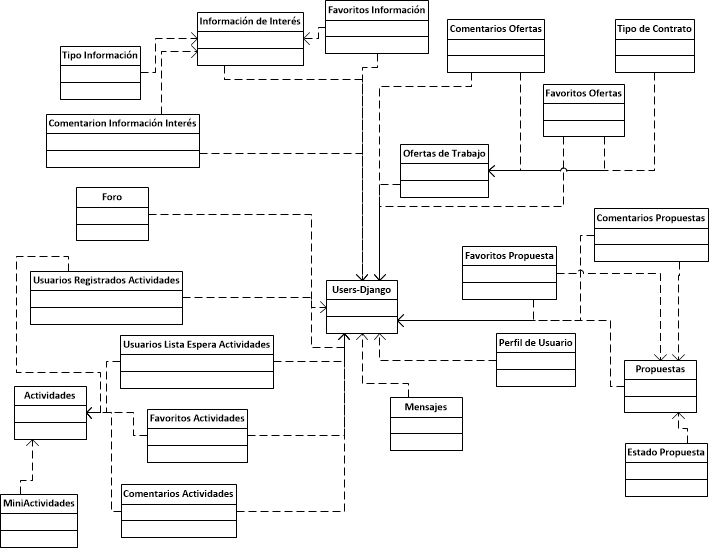
\includegraphics[width=12cm]{img/bbdd}
    \caption{Esquema de la Base de datos}
    \label{figura:basedatos}
 \end{figure}


 

A continuación se enumeran y describen cada una de las aplicaciones que utilizan la base de datos mostrada en la \figurename{basedatos}:


\begin{itemize}
\item Theme: en esta aplicación se define la estructura que tendrá la \textit{homepage}, también incluyen modelos para la creación de FAQs y la creación de un blog y sus respectivas entradas.

\item Propuestas: con esta aplicación conseguimos que los usuarios propongan sus propias actividades o al tipo de actividades que desean asistir.

Los campos contenidos en la base de datos para la clase Propuestas son:
	\begin{itemize}
		\item usuario
		\item titulo
		\item descripcion
		\item archivo
		\item estado\_propuesta que podrá ser Enviado, Aceptado o Rechazado
	\end{itemize}
	
\item Ofertas: con esta aplicación conseguimos dar a conocer las ofertas de trabajo y prácticas en empresas.

Los campos contenidos en la base de datos para la clase OfertasDeTrabajo son:
	\begin{itemize}
		\item titulo
		\item usuario
		\item descripcion
		\item como\_aplicar
		\item cuando
		\item donde
		\item url
		\item salario
		\item fichero
		\item tipo\_contrato que podrá ser Prácticas, Indefinido u Otros
	\end{itemize}
	
\item Actividades: con esta aplicación conseguimos dar a conocer las distintas actividades que se realizan en la Universidad. Estas actividades van desde un simple seminario o charla hasta actividades un poco más grandes como podría ser un taller con varios seminarios o incluso la organización y difusión de la semana de San Teleco.

Los campos contenidos en la base de datos para la clase Actividades son:
	\begin{itemize}
		\item usuario
		\item titulo
		\item descripcion
		\item archivo
		\item estado\_propuesta 
		\item fecha\_inicio
		\item fecha\_fin
		\item destacado: con este campo se indica que es una actividad importante, colocándola al principio de la lista
		\item url
		\item  lugar
		\item limite\_participantes: con este campo se decide si hay aforo limitado o no
		\item limit: si existiera aforo, con este campo delimitamos el número de personas registradas
		\item permitir\_inscriptions: con este campo se especifica si se aceptan inscripciones
		\item fecha\_inscripcion\_inicio
		\item fecha\_inscripcion\_final
		\item lista\_espera: con este campo se decide si se acepta poseer lista de espera		
		\item creditos\_rac: con este campo se decide si se conceden créditos RAC
		\item n\_rac: este campo especifica el número de créditos RAC que se conceden
		\item adminlist: en este campo se especifican los usuarios que participan en la organización de la actividad
		\item email\_organizador
		\item incluir\_miniactividades: con este campo se decide si se acepta poder incluir miniactividades
	\end{itemize}	
	
Tanto para la clase UsuariosRegistradosActividades como para la clase UsuariosListaEsperaActividades los campos que contienen sus bases de datos son los siguientes:
	\begin{itemize}
		\item actividad
		\item usuario
		\item fecha\_registro
		\item fecha\_actualizacion
	\end{itemize}
	
Los campos contenidos en la base de datos para la clase MiniActividad son:
	\begin{itemize}
		\item actividad
		\item titulo
		\item descripcion
		\item archivo
		\item lugar
		\item fecha
		\item hora
	\end{itemize}

\item Información de interés: con esta aplicación conseguimos difundir el resto de información que se desee compartir como becas, cursos, concursos, etc. 

Los campos contenidos en la base de datos para la clase InformacionInteres son:
	\begin{itemize}
		\item usuario
		\item titulo
		\item descripcion
		\item archivo
		\item cuando
		\item donde
		\item url
		\item tipo\_informacion que podrá ser Beca, Programa, Curso, Concurso u Otros
	\end{itemize}
	
\item Perfil: con esta aplicación conseguimos complementar el modelo de usuario creado por Django.
El modelo de Perfil creado debe referenciar a un usuario, pero no puede existir más de un perfil por usuario. 
No se mostrará públicamente algunos datos de carácter personal debido a la ley de protección de datos.

Los campos contenidos en la base de datos para la clase Profile son:
	\begin{itemize}
		\item usuario
		\item dni: este campo sólo se mostrará al registrarse en una actividad, y/o cuando se visite el propio perfil
		\item bio
		\item lugar
		\item foto 
		\item telefono
		\item pagina\_web
	\end{itemize}
	
Los campos contenidos en la base de datos para la clase ProfileProfesor son:
	\begin{itemize}
		\item usuario
		\item departamento
		\item puesto
		\item formacion
		\item investigacion
	\end{itemize}
	
Los campos contenidos en la base de datos para la clase ProfileAlumno son:
	\begin{itemize}
		\item usuario
		\item grado
		\item curso
	\end{itemize} 

Para todas las clases relacionadas con los Likes, los campos que contienen sus bases de datos son los siguientes:
	\begin{itemize}
		\item page
		\item usuario
	\end{itemize}

Para todas las clases relacionadas con los Comentarios y el Foro, los campos que contienen sus bases de datos son los siguientes:
	\begin{itemize}
		\item page
		\item usuario
		\item titulo
		\item comentario
		\item anonimo: con este campo se decide si un comentario es anónimo o no. En el foro, esta variable siempre será False
		\item archivo
		\item fecha
	\end{itemize}

Para la clase Mensajes, los campos que contienen su base de datos son los siguientes:
\begin{itemize}
		\item destinatario
		\item remitente
		\item subject
		\item body
		\item fecha
	\end{itemize}    
    
\item BasicModels y BasicContent: estas dos aplicaciones han sido creadas para proporcionar una base para dos propósitos:
\begin{itemize}
\item Crear páginas básicas como las creadas para mostrar las listas de ofertas, información de interés, etc.
\item Extender el modelo al crear los modelos anteriormente comentados unificando en uno solo los campos comunes, además de proporcionar \textit{templates} comunes para el resto de aplicaciones.
Con estas dos aplicaciones conseguimos reducir el código, evitando en la medida de lo posible la repetición del mismo.
\end{itemize}
\end{itemize}


\subsection{Tipo de usuarios} 
\label{subsec:usuarios}


Dentro de la aplicación se distinguen tipos de usuarios, con distintos roles y diferentes permisos:

\begin{itemize}
\item No registrados: Estos usuarios sólo pueden ver el contenido de la aplicación pero no pueden interactuar ni con la aplicación ni con otros usuarios.
\item Alumnos: Este tipo de usuarios además de ver el contenido, pueden interactuar con la aplicación, lo único que no pueden hacer es crear actividades, aunque podrían editarlas y eliminarlas si formaran parte de la administración en alguna de ellas.
\item Profesores: Este tipo de usuarios además de lo que los alumnos pueden hacer también pueden crear actividades y cambiar el estado de una propuesta.
\item Administradores: Además de todo lo descrito anteriormente. Tiene acceso a la parte de administración.
\end{itemize}


\subsection{Amazon Web Service + Apache} 
\label{subsec:aws_apache}
La aplicación se ha desplegado en una máquina EC2 de Amazon Web Service usando una cuenta gratuita para estudiantes de duración de un año.

Para crear la máquina se ha escogido las siguientes opciones:\\
- El sistema operativo es: Ubuntu 14.04 LTS con una capacidad total de 8GB.\\
- Una instancia de tipo t2.micro: 1 GiB de memoria, 1 vCPU solo para EBS y plataforma de 32 bits o 64 bits. Las instancias T2 son instancias de desempeño con ráfagas que proporcionan un nivel base de desempeño de la CPU con la posibilidad de alcanzar ráfagas por encima del nivel básico. Las instancias de este tipo son ideales para aplicaciones que no usan la CPU por completo, a menudo o de manera constante, pero que de vez en cuando tienen que alcanzar ráfagas (por ejemplo, servidores web, entornos para desarrolladores y bases de datos). En este caso es una máquina de 64bits.

En las siguientes imágenes se pueden ver las diferentes características de la máquina creada:
\begin{figure}[H]
   \centering
   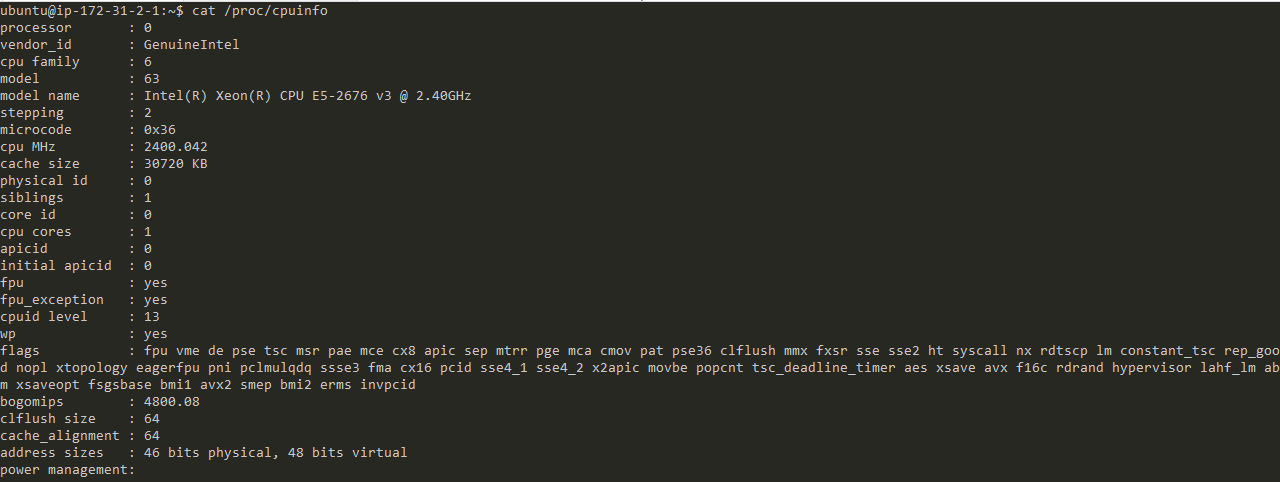
\includegraphics[width=12cm]{img/cpuinfo}
   \caption{Salida de la ejecución del comando cat /proc/cpu/info }
   \label{figura:cpuinfo}
\end{figure}
\begin{figure}[H]
   \centering
   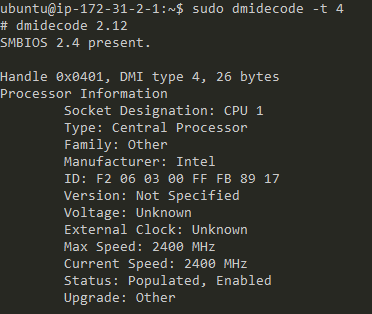
\includegraphics[width=12cm]{img/dmidecode}
   \caption{Salida de la ejecución del comando sudo demidecode -t 4}
   \label{figura:dmidecode}
\end{figure}
\begin{figure}[H]
   \centering
   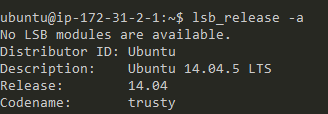
\includegraphics[width=12cm]{img/lsb_release}
   \caption{Salida de la ejecución del comando lsb\_release -a}
   \label{figura:lsb_release}
\end{figure}
\begin{figure}[H]
   \centering
   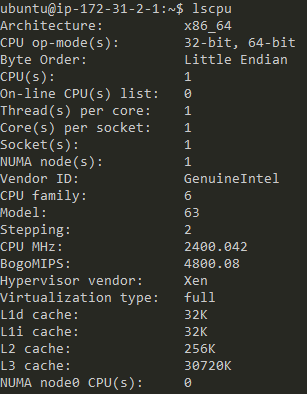
\includegraphics[width=12cm]{img/lscpu}
   \caption{Salida de la ejecución del comando lscpu}
   \label{figura:lscpu}
\end{figure}
\begin{figure}[H]
   \centering
   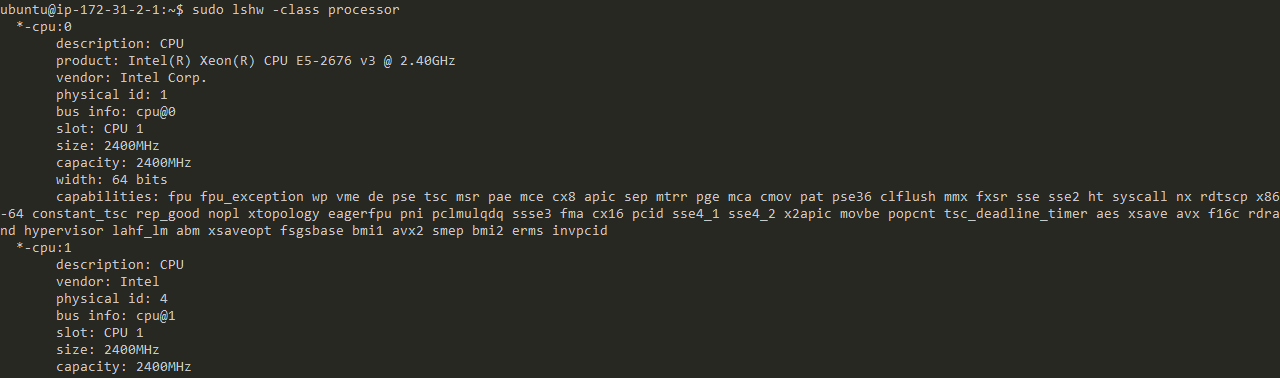
\includegraphics[width=12cm]{img/lshw}
   \caption{Salida de la ejecución del comando lshw}
   \label{figura:lshw}
\end{figure}
\begin{figure}[H]
   \centering
   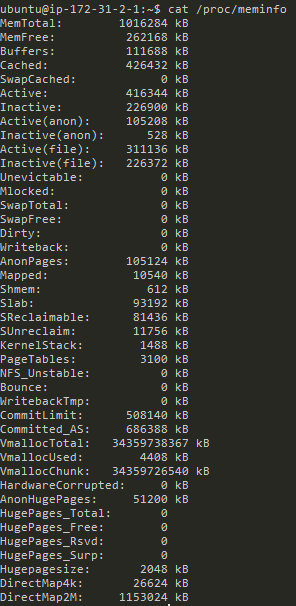
\includegraphics[width=12cm]{img/meminfo}
   \caption{Salida de la ejecución del comando cat /proc/meminfo}
   \label{figura:meminfo}
\end{figure}


Para la configuración de Apache, primero se debe instalar usando el comando: 

\begin{verbatim}
	apt-get install apache2
\end{verbatim}

Para poder servir aplicaciones Django desde un servidor Apache, lo más habitual es añadir el módulo mod\_wsgi, que permite servir aplicaciones hechas en Python, que tengan soporte para la interfaz WSGI (Como es el caso de Django y en este caso también de Mezzanine).


Para ello se instala el paquete del repositorio:
\begin{verbatim}
	sudo apt-get install libapache2-mod-wsgi
\end{verbatim}

A continuación se configuró el host virtual de Apache. Un virtual host permite mantener múltiples nombres de host en Apache. Gracias a ello, se puede decirle a Apache que redirija las peticiones procedentes de una URL determinada, a una aplicación concreta.

Para generar la configuración del host virtual, se creó un archivo en /etc/apache2/sites-available/ con el nombre de Welpe.

La configuración usada se muestra en la siguiente captura:

\begin{figure}[H]
   \centering
   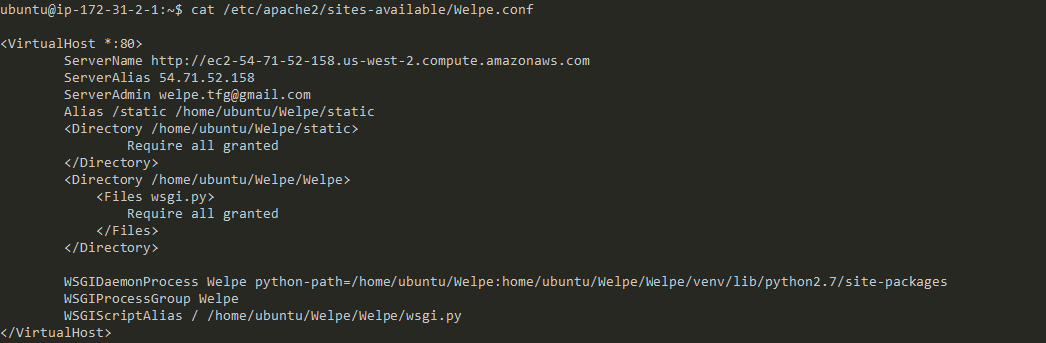
\includegraphics[width=12cm]{img/welpe_conf}
   \caption{Fichero de configuración en Apache}
   \label{figura:welpe_conf}
\end{figure}

Después de configurar el anterior fichero, se activó el host virtual y se reinició el servidor mediante:
\begin{verbatim}
	sudo a2ensite Welpe
	sudo /etc/init.d/apache2 restart
\end{verbatim}


\section{Diseño e implementación del cliente} 
\label{sec:cliente}
El cliente puede acceder a la interfaz web a través de un navegador web. Como bien se ha comentado anteriormente, se han utilizado distintas tecnologías para que la interfaz sea más amigable. HTML5 y CSS3 junto con Bootstrap y jQuery han sido necesarias para definir cómo se visualizan y con qué estilos y diseños aparecen cada uno de los elementos visibles en esta aplicación. \\
Todas las vistas de este proyecto siguen el mismo esquema:
\begin{itemize}
\item Una barra superior o \textit{header} que consta del logotipo de la aplicación junto con el login y un formulario de búsqueda. Además también consta del menú y ya por último se ha introducido también otra pequeña cabecera con el nombre de vista junto con lo que llamaríamos \textit{breadcrumb} o migas de pan.  Breadcrumb es un elemento que aporta al usuario la información de dónde se encuentra en cada momento dentro de un sitio web. Se indica la ubicación exacta de la página y la relación jerárquica de esta con respecto a la de inicio del sitio web.
\item Contenido principal de la página. En esta sección lo que nos encontramos es con el contenido renderizado que estamos pidiendo a través de la URL introducida ya sea el perfil de usuario, una actividad, una oferta o cualquier otra petición.
\item Footer. En el footer podemos encontrar el copyright®, política de cookies, etc.
\end{itemize}

\subsection{Vistas de las páginas} 
\label{subsec:vistas}
A continuación se describen una a una todas las páginas de la aplicación explicando cada elemento que aparece en las páginas así como su utilidad. Todas las páginas en principio son públicas y accesibles para todo tipo de usuarios tanto para los registrados como para los no registrados aunque también se ha de decir, que estando registrado en esta aplicación, se puede interactuar por ejemplo escribiendo comentarios, creando propuestas, etc., además si en un futuro esta aplicación se expandiera podría tener contenido exclusivo sólo para usuarios registrados.

\subsubsection{Página de inicio}
\label{subsubsec:home}
\begin{figure}[H]
\centering
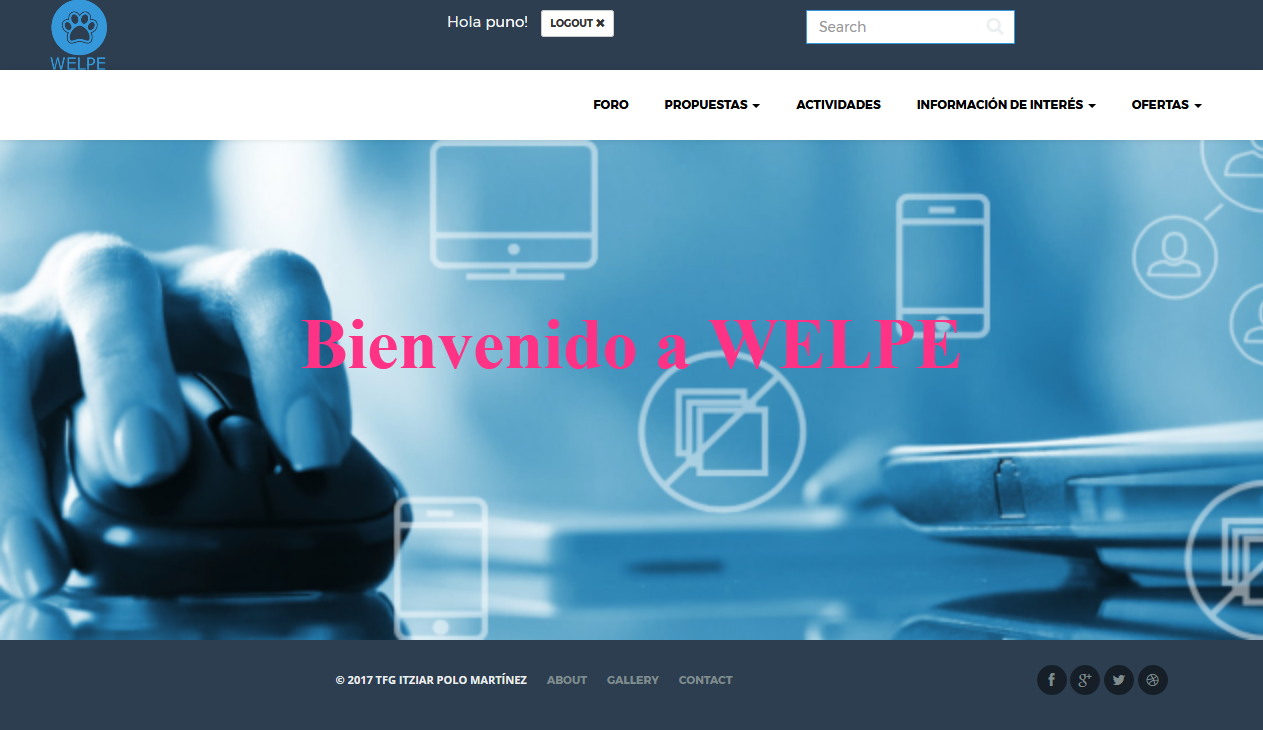
\includegraphics[width=12cm]{img/home}
\caption{Hompage}
\label{figura:home}
\end{figure}
La página de inicio es enviada al cliente cuando se recibe una petición GET sobre el recurso /, a través de la vista home. En esta vista hace un resumen de las características que tiene la aplicación web.

\subsubsection{Página del Perfil de Usuario}
\label{subsubsec:profile}
\begin{figure}[H]
\centering
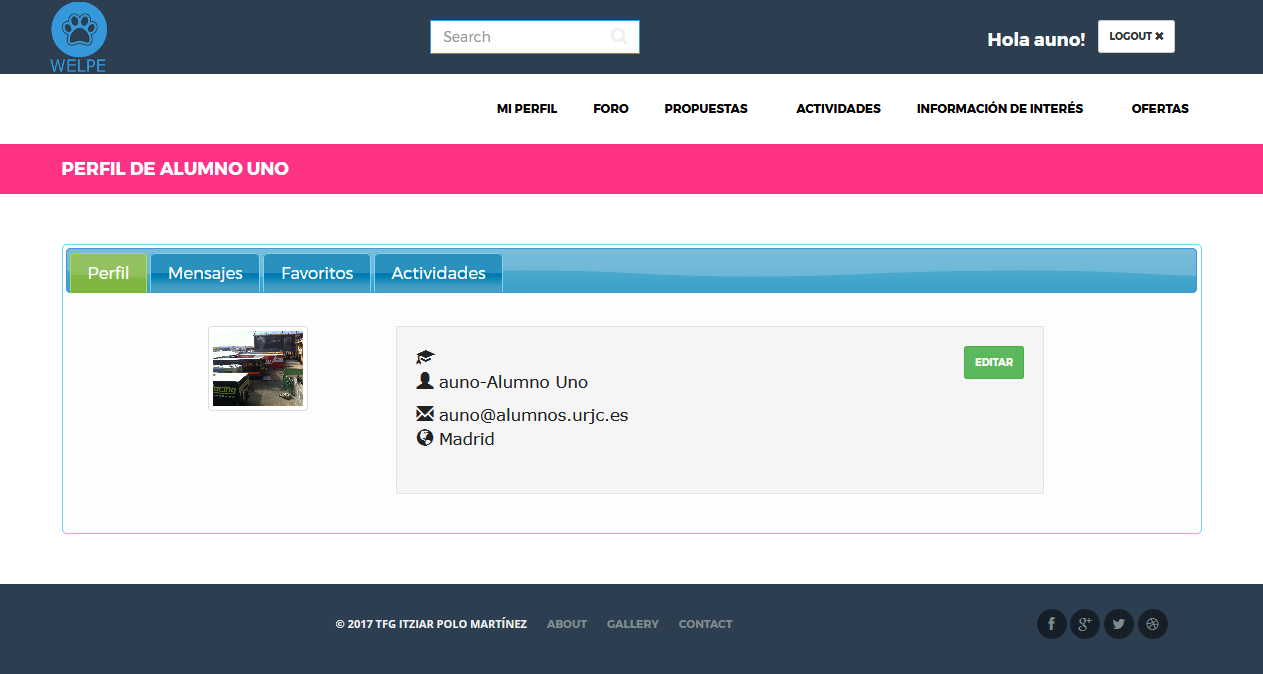
\includegraphics[width=12cm]{img/mi_perfil}
\caption{Vista del perfil de usuario}
\label{figura:perfil_usuario}
\end{figure}
\begin{figure}[H]
\centering
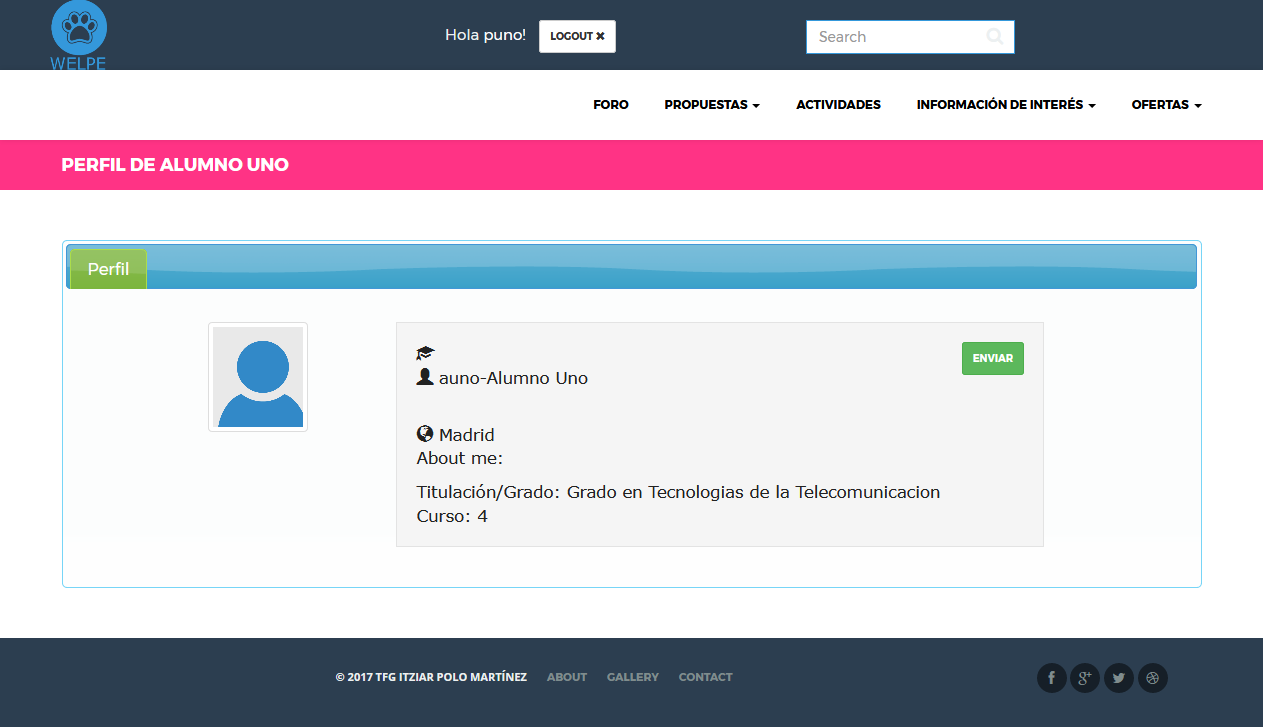
\includegraphics[width=12cm]{img/perfil_otro}
\caption{Vista del perfil de otro usuario distinto}
\label{figura:perfil_otro_usuario}
\end{figure}
\begin{figure}[H]
\centering
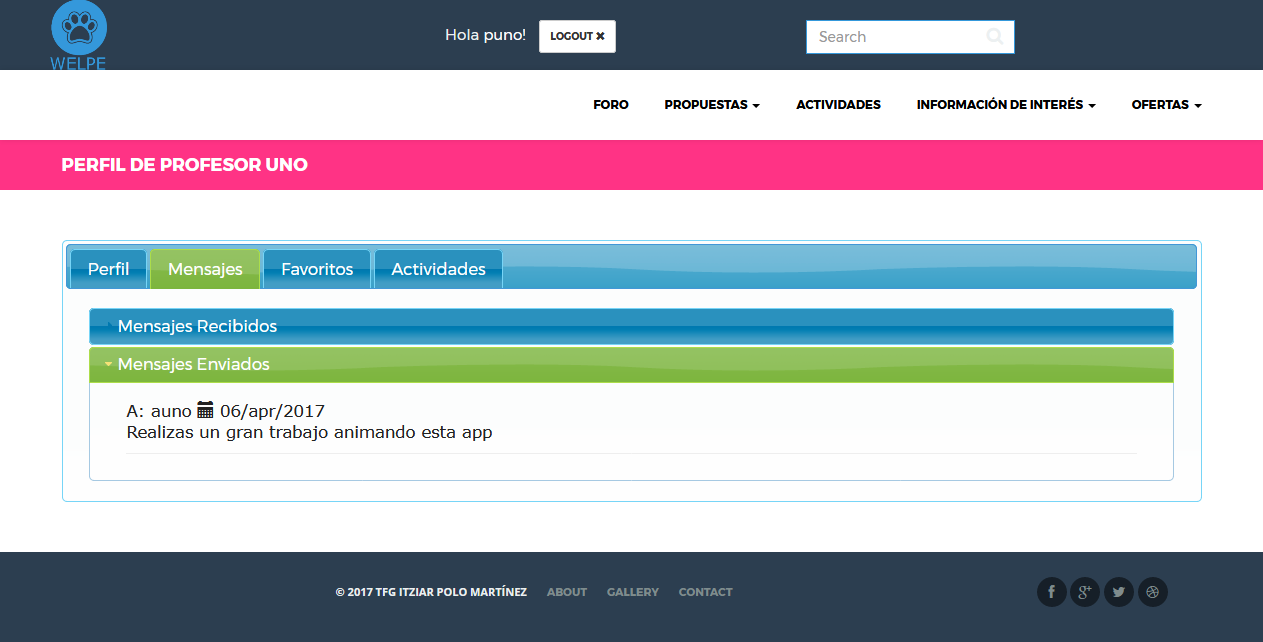
\includegraphics[width=12cm]{img/perfil_mensajes}
\caption{Vista de los mensajes}
\label{figura:perfil_mensajes}
\end{figure}
\begin{figure}[H]
\centering
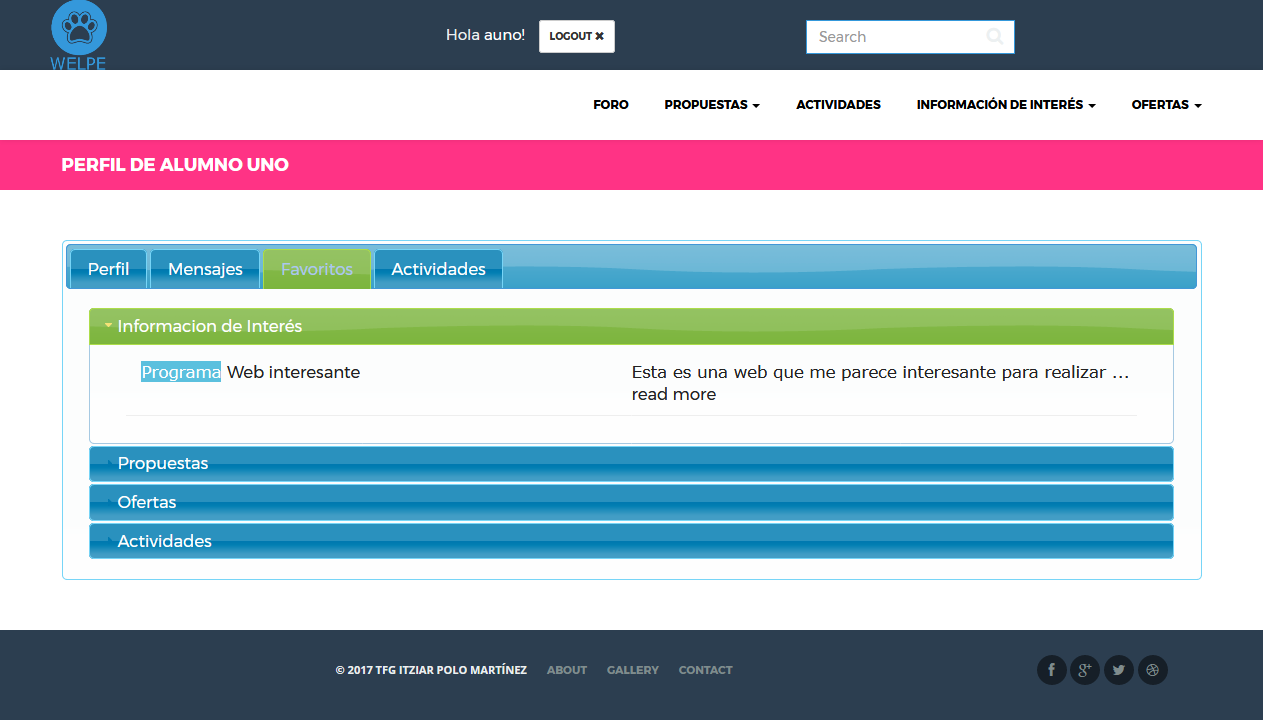
\includegraphics[width=12cm]{img/perfil_favoritos}
\caption{Vista de favoritos}
\label{figura:perfil_favoritos}
\end{figure}
\begin{figure}[H]
\centering
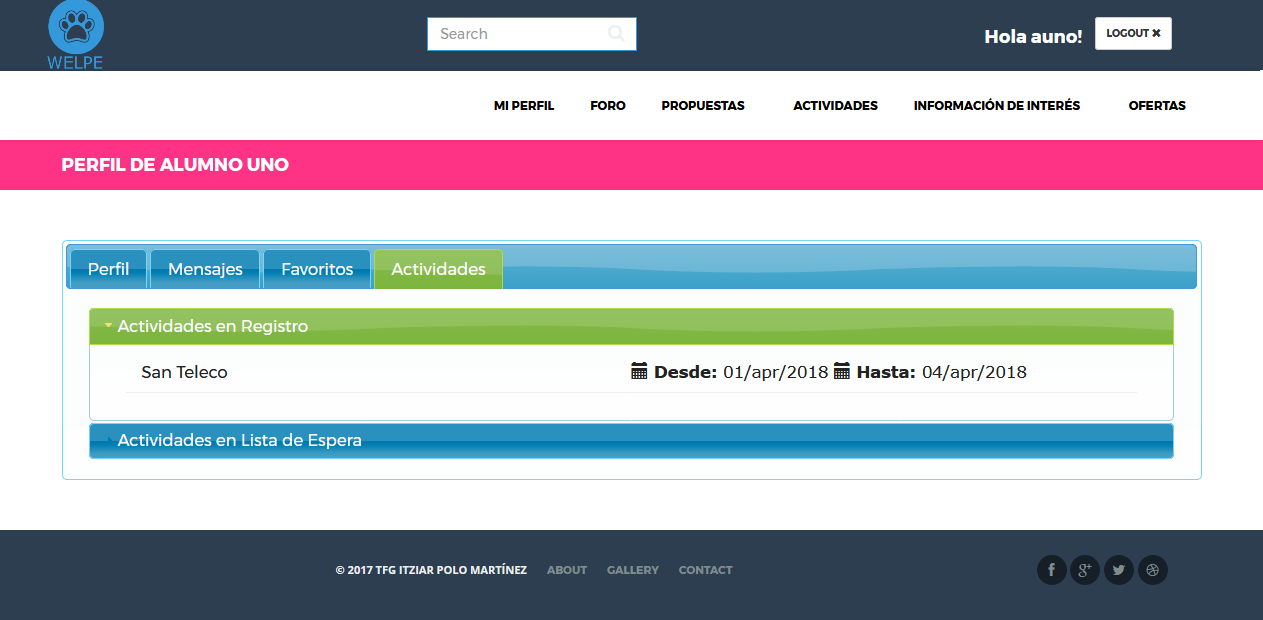
\includegraphics[width=12cm]{img/perfil_actividades}
\caption{Vista de actividades registradas}
\label{figura:perfil_actividades}
\end{figure}
La página del perfil es enviada al cliente cuando se recibe una petición GET sobre el recurso /perfil/{id\_usuario}.\\
En esta vista se muestra la información de un usuario.\\
El contenido dependerá de si un usuario accede a su propio perfil o al perfil de otro usuario.\\
Aquí nos encontramos varias cosas:
\begin{itemize}
\item El perfil de usuario que además de la información del usuario, se podrá interactuar con él, enviándole un mensaje privado.
\item Si se accede al propio perfil, se podrá además de editarlo, tener acceso a la lista de mensajes tanto enviados como recibidos, a la lista de favoritos ordenados por cada uno de los eventos y ver las actividades en las que se desea participar.
\end{itemize} 

\subsubsection{Página del Foro}
\label{subsubsec:foro}
\begin{figure}[H]
\centering
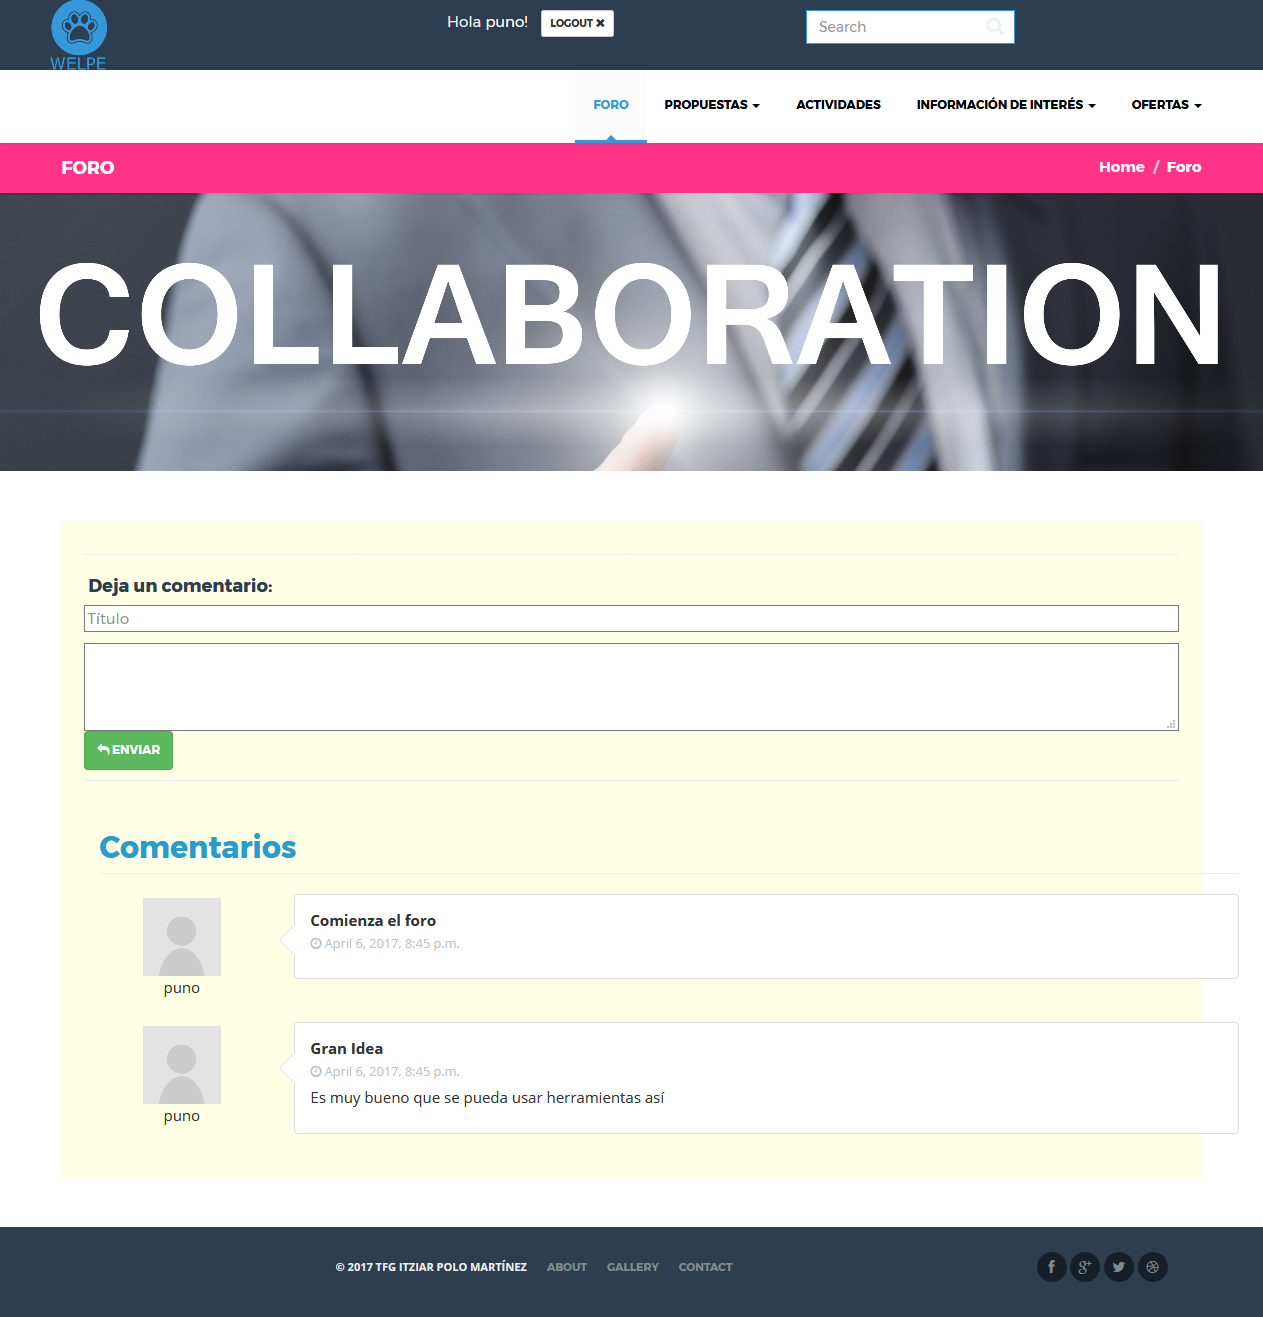
\includegraphics[width=12cm]{img/foro}
\caption{Vista del foro}
\label{figura:foro}
\end{figure}
La página del foro es enviada al cliente cuando se recibe una petición GET sobre el recurso /foro.\\
La página foro contiene todos los mensajes publicados en el foro.\\
Cada mensaje contiene la foto y el nombre del usuario (aunque estos datos pueden ser anónimos), la fecha en la que se publicó, un título de comentario, una descripción (que será opcional).\\
Encima de estos mensajes al igual que en las demás vistas que contienen comentarios aparece un formulario para si se desea dejar un comentario.\\
El objetivo inicial del foro era dotar a la aplicación de un aspecto más social según lo comentado en los objetivos.\\
La función del foro es la de conectar a todos los usuarios, permitiendo un entorno universitario conectado y permitiendo mejorar el mismo, por ejemplo compartiendo curiosidades que los usuarios vayan encontrando durante su estancia en la universidad.

\subsubsection{Página de Propuestas}
\label{subsubsec:propuestas}
\begin{figure}[H]
\centering
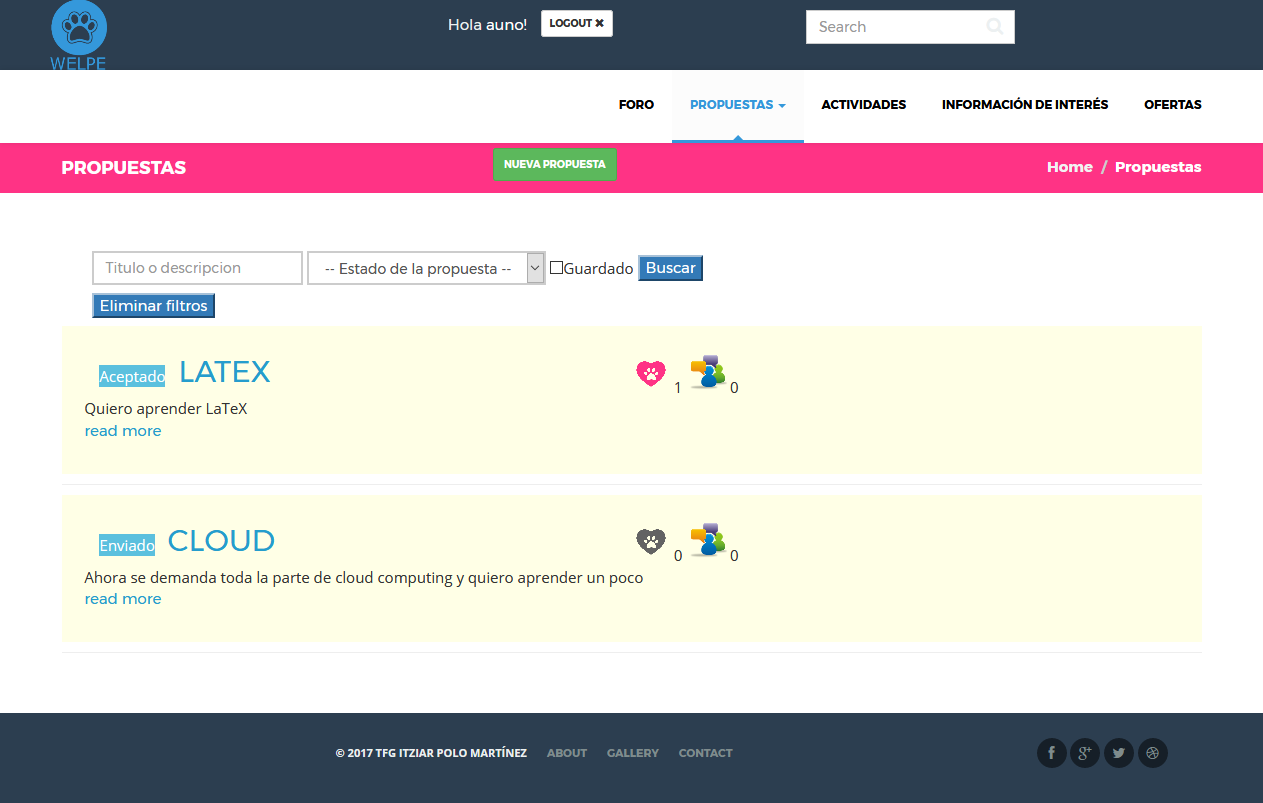
\includegraphics[width=12cm]{img/propuestas}
\caption{Vista de la lista de propuestas}
\label{figura:propuestas}
\end{figure}
La página del listado de propuestas es enviada al cliente cuando se recibe una petición GET sobre el recurso /propuestas.\\
En esta vista se proporciona un listado con todas las propuestas que se han ido recopilando, junto con una pequeña parte de la descripción. Además a la izquierda del título se muestra el estado de la propuesta y a la derecha se puede observar varios elementos. En primer lugar un corazón que viene a significar si la propuesta se ha guardado en la lista de favoritos o no, además de un número que irá creciendo o decreciendo dependiendo del número de usuarios la guarden en sus listas de favoritos. A continuación se observa el número de comentarios que contiene cada una de las ofertas.\\
También cualquier usuario (registrado o no) puede filtrar las propuesta por las palabras que contenga el título o contenido de la propuesta, además también se puede filtrar por el estado de las propuestas a elegir entre enviado, aceptado o rechazado, además si el usuario está registrado podrá filtrar si la propuesta está o no en su lista de favoritos.\\
Para introducir una nueva propuesta cualquier usuario registrado puede hacerlo. Para ello, se rellena el formulario con los datos correspondientes y envía ese formulario. Esta petición llega al servidor mediante una petición POST donde se encargará de sacar los datos y guardarlos correctamente en la base de datos, devolviendo como resultado una nueva vista donde se muestra la nueva propuesta.\\
Por último, sólo si el usuario ha creado una determinada propuesta o es un profesor o es el administrador: podrá modificar y/o eliminar dicha propuesta mediante los botones edit y delete.

\subsubsection{Página de una Propuesta}
\label{subsubsec:propuesta}
\begin{figure}[H]
\centering
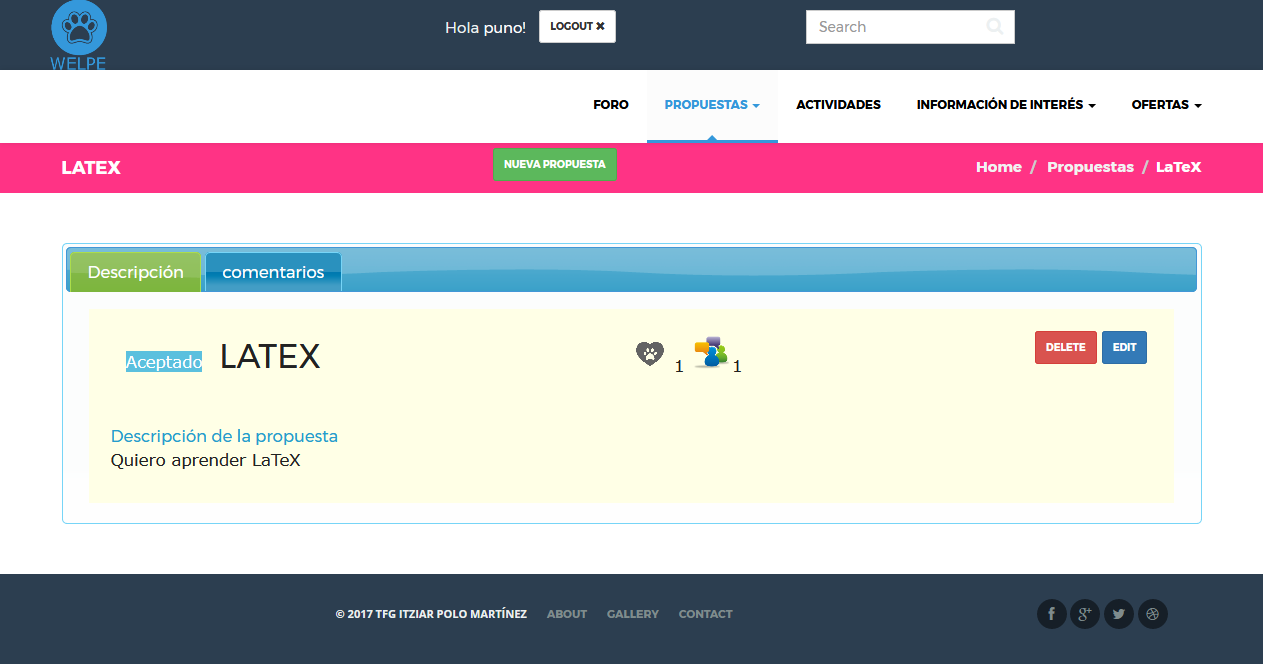
\includegraphics[width=12cm]{img/propuesta}
\caption{Vista de una propuesta}
\label{figura:propuesta}
\end{figure}
\begin{figure}[H]
\centering
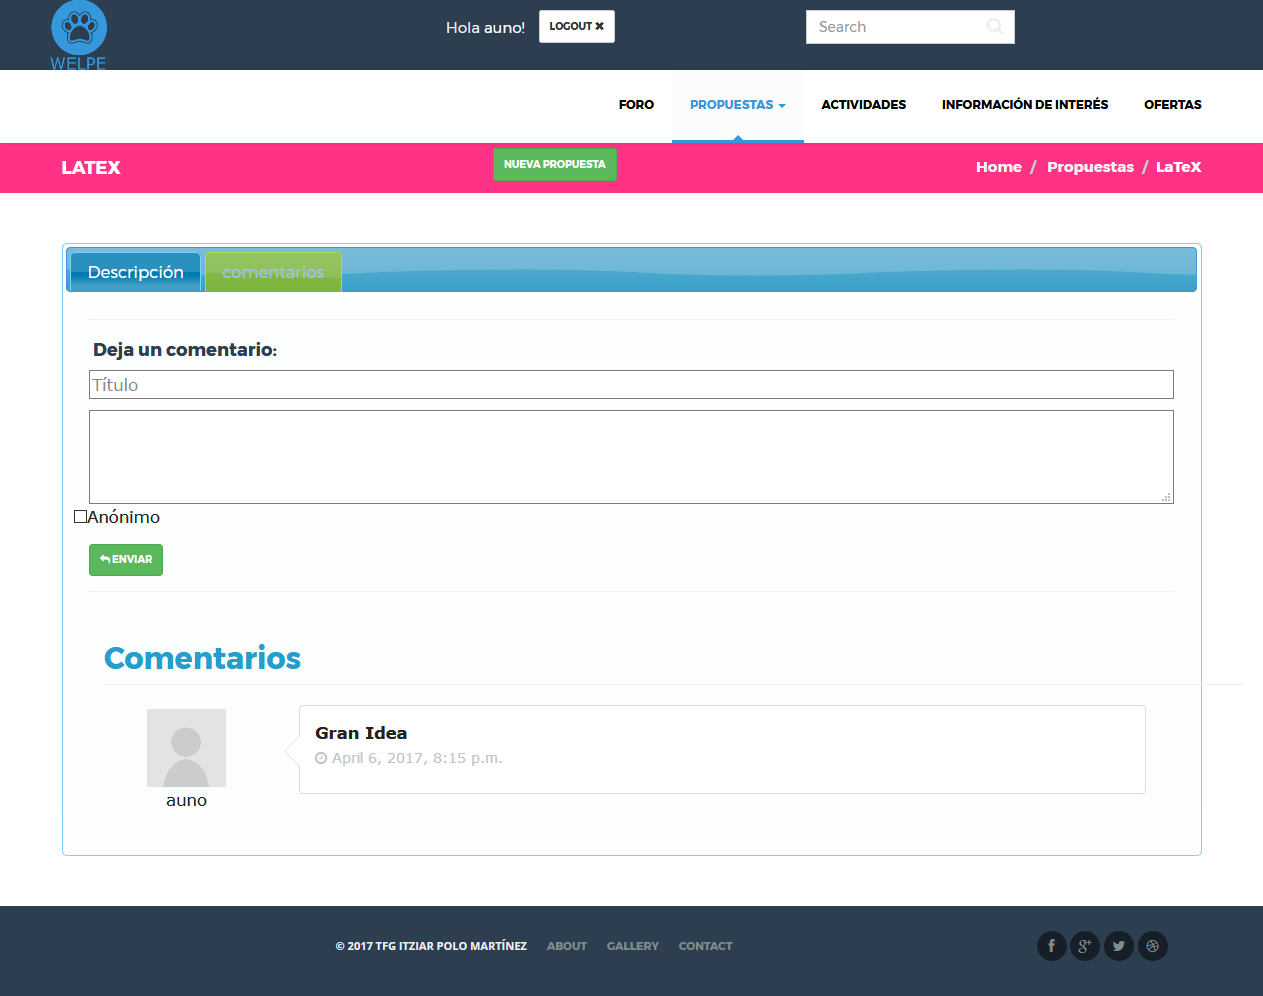
\includegraphics[width=12cm]{img/propuesta_comment}
\caption{Vista de los comentarios a una propuesta}
\label{figura:propuesta_comment}
\end{figure}
La página de una propuesta es enviada al cliente cuando se recibe una petición GET sobre el recurso /propuestas/{título\_propuesta}\\
En esta vista se muestra toda la información relativa a la propuesta previamente introducida a través del formulario comentado anteriormente.\\
Relativo a esta vista, se encuentra el nombre, el estado de la propuesta, número de comentarios, los comentarios, la popularidad que se mide en el número de favoritos, etc.\\
En esta vista se puede interactuar de las siguientes formas sólo si es un usuario registrado:
\begin{itemize}
\item Se puede crear una nueva propuesta mediante el botón nueva propuesta donde se abrirá un modal en el que se pedirán ciertos datos; este formulario ya cumplimentado se enviará al servidor donde se procesará y almacenara devolviendo como resultado una nueva vista donde se muestra la nueva propuesta que el usuario ha creado.
\item Si el usuario es el propietario de la propuesta podrá modificarla mediante el botón edit y también podrá eliminarla mediante el botón eliminar.
\item Junto con todo ello, está también el botón de favoritos donde el usuario puede agregar o eliminar la propuesta de su lista de favoritos.  
\item Se ha proporcionado un apartado de comentarios a la propuesta para que los usuarios puedan comentar cada propuesta.
\item Sólo los profesores y el administrador pueden cambiar el estado de la propuesta. Esto es así, ya que el objetivo de las propuestas es que los alumnos den opinión de qué es lo que quieren aprender en los seminarios y/o proponer ellos mismos los seminarios que quieren impartir.
\end{itemize}

\subsubsection{Página de Actividades}
\label{subsubsec:actividades}
\begin{figure}[H]
\centering
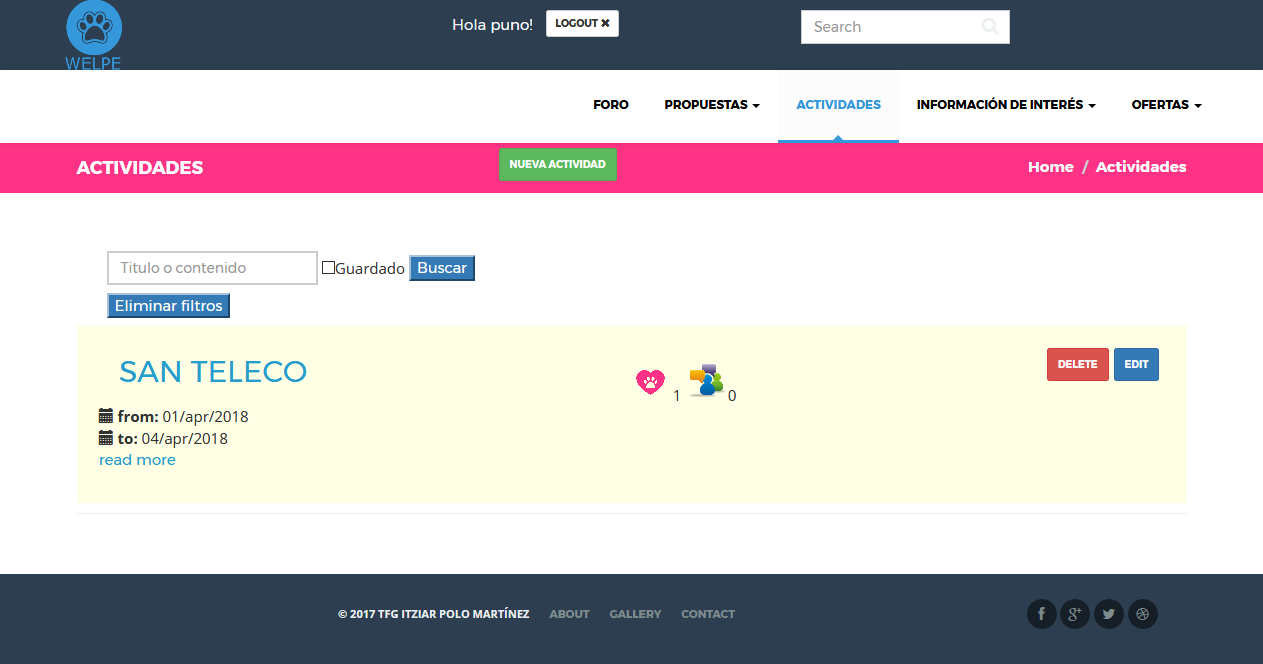
\includegraphics[width=12cm]{img/actividades}
\caption{Vista de la lista de actividades}
\label{figura:actividades}
\end{figure}
La página del listado de actividades es enviada al cliente cuando se recibe una petición GET sobre el recurso /actividades.\\
En esta vista se muestra un listado con todas las actividades que han ido recopilando junto con una pequeña parte de la descripción. Se puede observar el título junto con varios elementos a la derecha. En primer lugar un corazón que viene a significar si la actividad se ha guardado en la lista de favoritos o no, además de un número que irá creciendo o decreciendo dependiendo del número de usuarios que guarden en sus listas de favoritos dichas actividades. A continuación se observa el número de comentarios que contiene cada una de las actividades.\\
También cualquier usuario (registrado o no) puede filtrar las actividades por las palabras que contenga el título o contenido de la actividad, además si el usuario está registrado, podrá filtrar el listado de las actividades, si la actividad está o no en su lista de favoritos.\\
Para introducir una nueva actividad, sólo los administradores y los profesores pueden hacerlo. Esto es así, ya que se necesita el consentimiento de un profesor para que un alumno pueda organizar una actividad. Para ello se rellena el formulario con los datos correspondientes y se envía ese formulario. Esta petición llega al servidor mediante una petición POST donde se encargará de sacar los datos y guardarlos correctamente en la base de datos, devolviendo como resultado una nueva vista donde se muestra la nueva actividad.\\
Por último, sólo si el usuario ha creado o está incluido en la lista de administradores de una determinada actividad o es un profesor o es el administrador: podrá modificar y/o eliminar dicha actividad mediante los botones edit y delete.

\subsubsection{Página de una Actividad}
\label{subsubsec:actividad}
\begin{figure}[H]
\centering
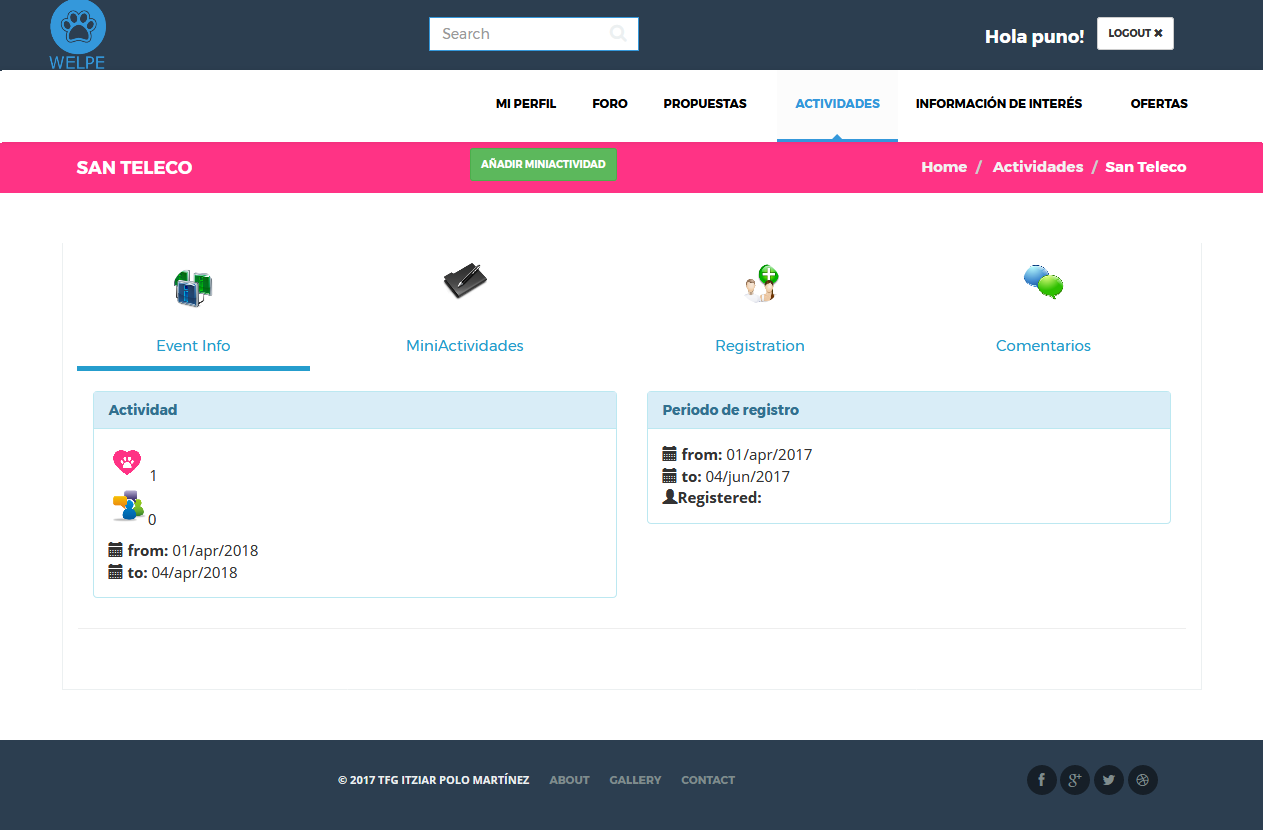
\includegraphics[width=12cm]{img/actividad}
\caption{Vista de una actividad}
\label{figura:actividad}
\end{figure}
\begin{figure}[H]
\centering
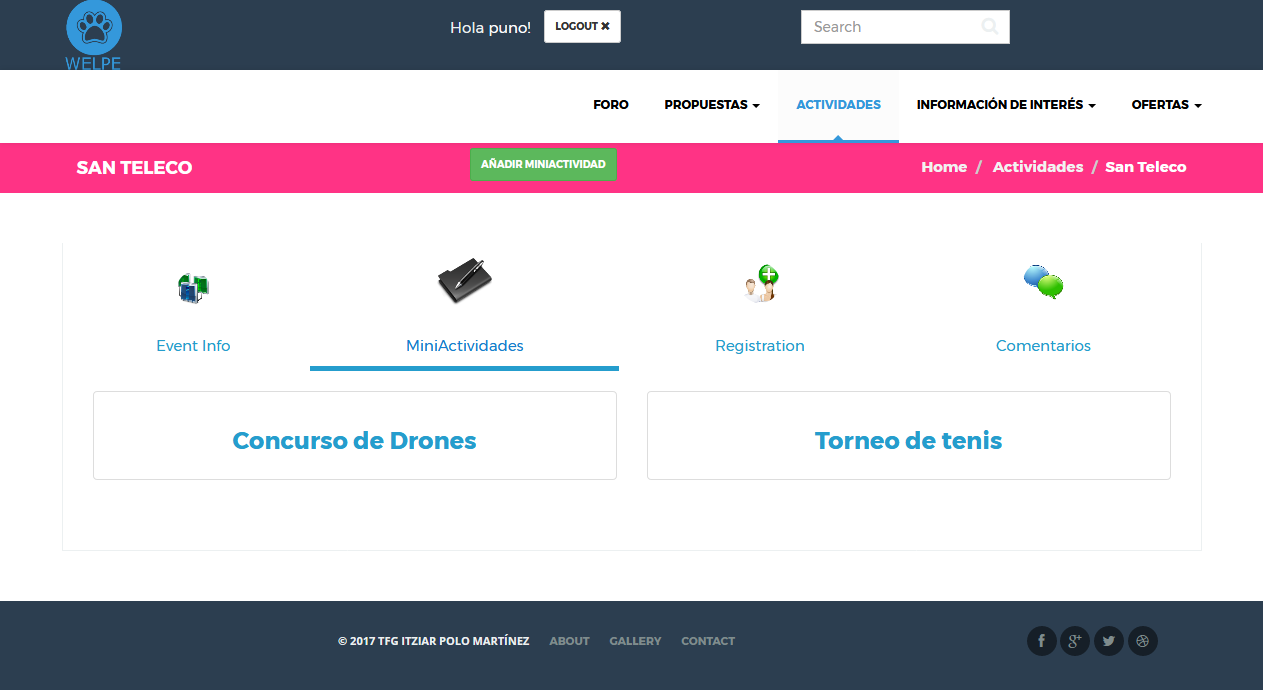
\includegraphics[width=12cm]{img/actividad_miniactividad}
\caption{Vista de las miniactividades}
\label{figura:actividad_miniactividad}
\end{figure}
\begin{figure}[H]
\centering
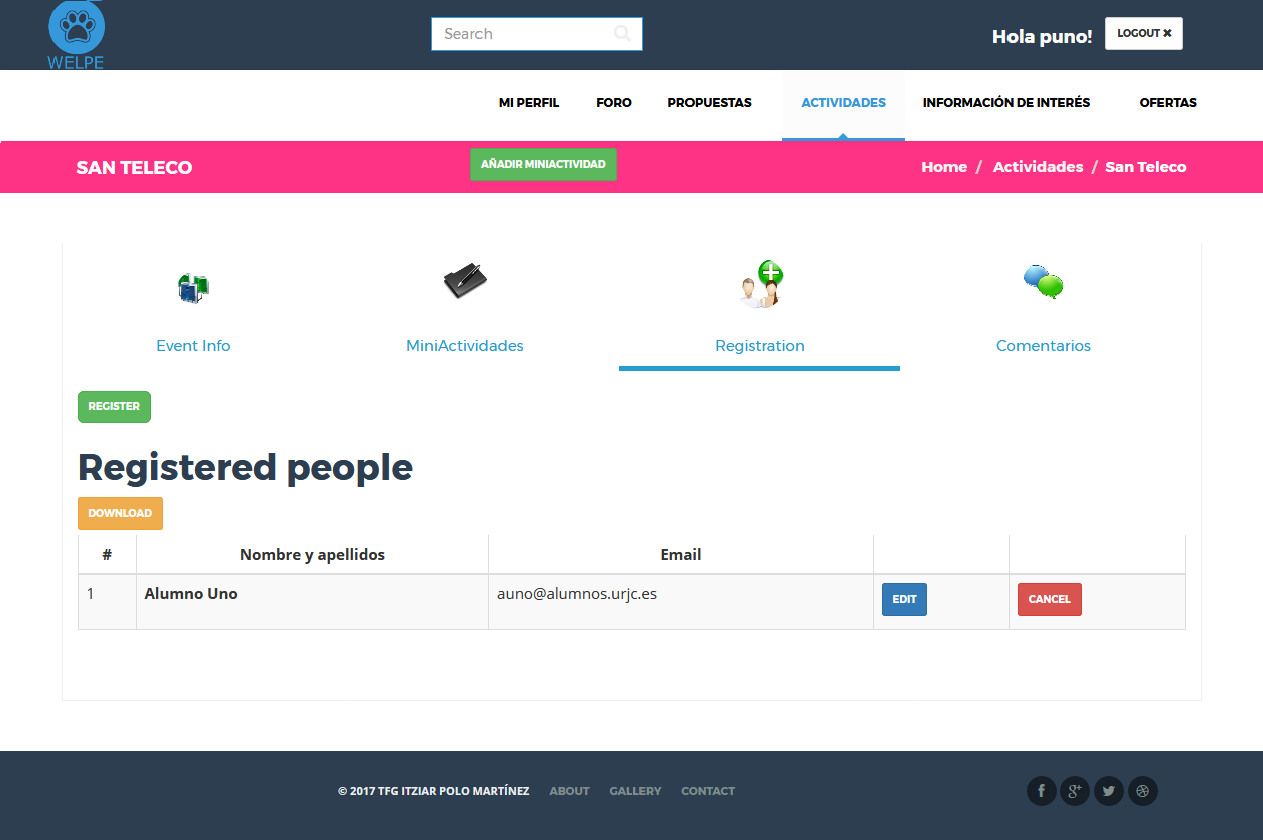
\includegraphics[width=12cm]{img/actividad_registro}
\caption{Vista del registro}
\label{figura:actividad_registro}
\end{figure}
\begin{figure}[H]
\centering
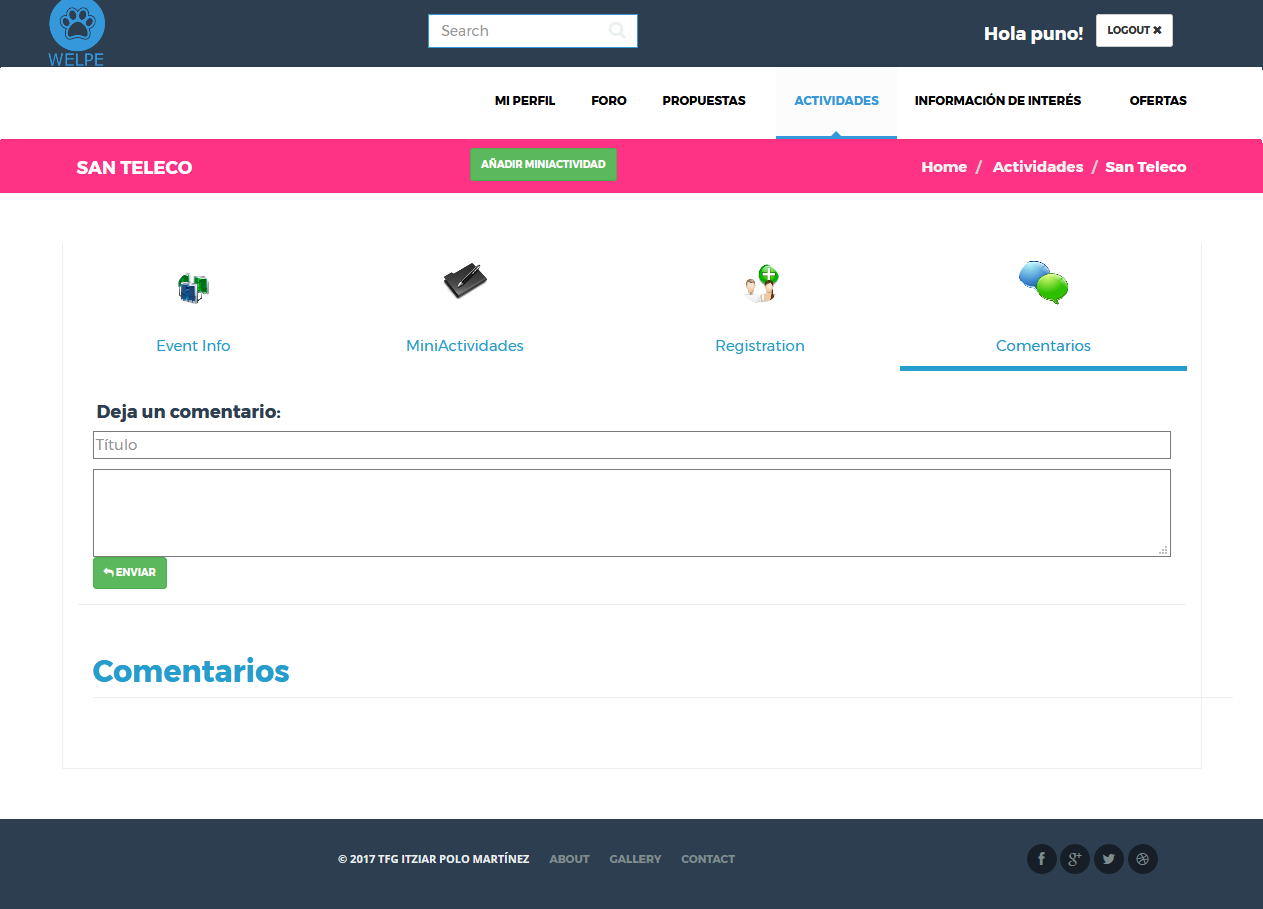
\includegraphics[width=12cm]{img/actividad_comment}
\caption{Vista de los comentarios a una actividad}
\label{figura:actividad_comment}
\end{figure}
La página de una actividad es enviada al cliente cuando se recibe una petición GET sobre el recurso /propuestas/{título\_actividad}\\
En esta vista se muestra toda la información relativa a la actividad previamente introducida a través del formulario comentado anteriormente.\\
Relativo a esta vista, se encuentra el nombre, numero de comentarios, los comentarios, la popularidad de la actividad basada en el número de favoritos, la descripción de la actividad, las fechas, etc.\\
En esta vista se puede interactuar de las siguientes formas, sólo si es un usuario registrado:
\begin{itemize}
\item Si la actividad incluye que se puedan incluir miniactividades. Se podrá crear miniactividades mediante el botón nueva miniactividad donde se abrirá un modal en el que se pedirán ciertos datos; este formulario ya cumplimentado se enviará al servidor donde se procesará y almacenara. Las miniactividades son actividades dentro de una gran actividad.  
\item Si la actividad proporciona un registro, la vista contendrá una pestaña de registro de usuarios. Donde los usuarios que deseen participar puedan inscribirse. Mientras que los administradores de la actividad pueden además ver y obtener la lista de participantes mediante la descarga de un archivo xls.
\item Se ha proporcionado un apartado de comentarios a la actividad para que los usuarios puedan comentar cada actividad.
\end{itemize}


\subsubsection{Página de Ofertas}
\label{subsubsec:ofertas}
\begin{figure}[H]
\centering
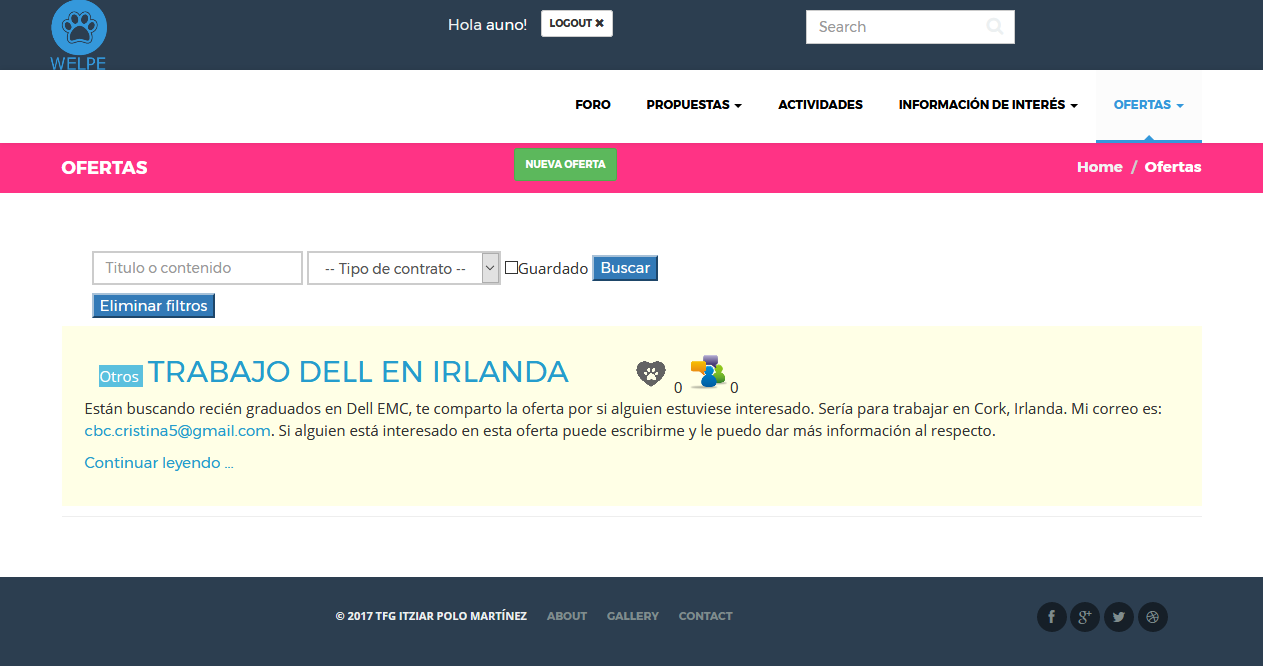
\includegraphics[width=12cm]{img/ofertas}
\caption{Vista de la lista de ofertas}
\label{figura:ofertas}
\end{figure}
La página del listado de ofertas es enviada al cliente cuando se recibe una petición GET sobre el recurso /ofertas.\\
En esta vista se muestra un listado con todas las ofertas que se han ido recopilando junto con una pequeña parte de la descripción. Además a la izquierda del título se muestra el tipo de contrato que se ofrece y a la derecha se puede observar varios elementos. En primer lugar un corazón que viene a significar si la oferta se ha guardado en la lista de favoritos o no, además de un número que irá creciendo o decreciendo dependiendo del número de usuarios que guarden en sus listas de favoritos dichas ofertas. A continuación se observa el número de comentarios que contiene cada una de las ofertas.\\
También cualquier usuario (registrado o no) puede filtrar las ofertas por la/s palabra/s que contenga el título o contenido de la oferta, además también se puede filtrar por el tipo de contrato que se ofrece a elegir entre contrato indefinido, prácticas u otro tipo de contratos y además si el usuario está registrado podrá filtrar si la oferta está o no en su lista de favoritos.\\
Para introducir una nueva oferta cualquier usuario registrado puede hacerlo. Para ello se rellena el formulario con los datos correspondientes y envía ese formulario. Esta petición llega al servidor mediante una petición POST donde se encargará de sacar los datos y guardarlos correctamente en la base de datos, devolviendo como resultado una nueva vista donde se muestra la nueva oferta.\\
Por último, sólo si el usuario ha creado una determinada oferta o es un profesor o es el administrador: podrá modificar y/o eliminar dicha oferta mediante los botones edit y delete.


\subsubsection{Página de una Oferta}
\label{subsubsec:oferta}
\begin{figure}[H]
\centering
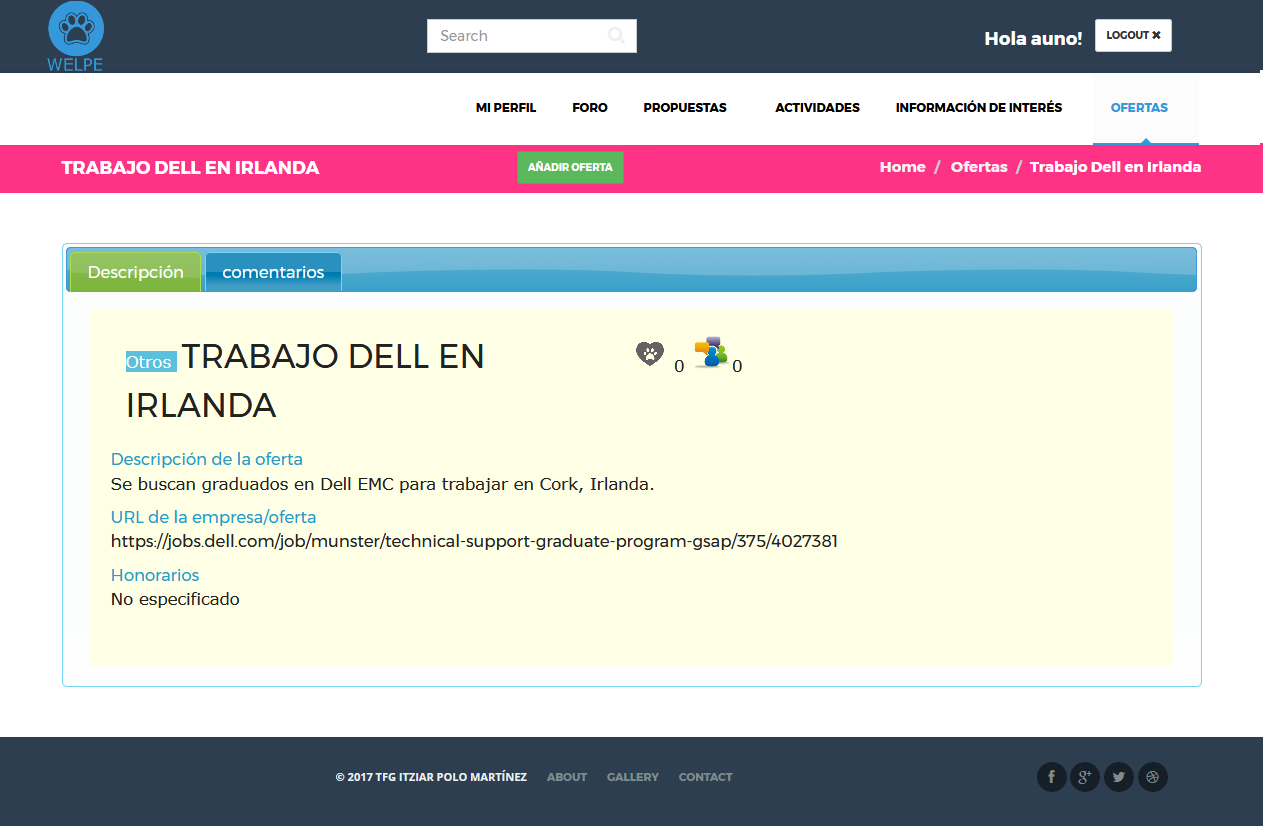
\includegraphics[width=12cm]{img/oferta}
\caption{Vista de una oferta}
\label{figura:oferta}
\end{figure}
\begin{figure}[H]
\centering
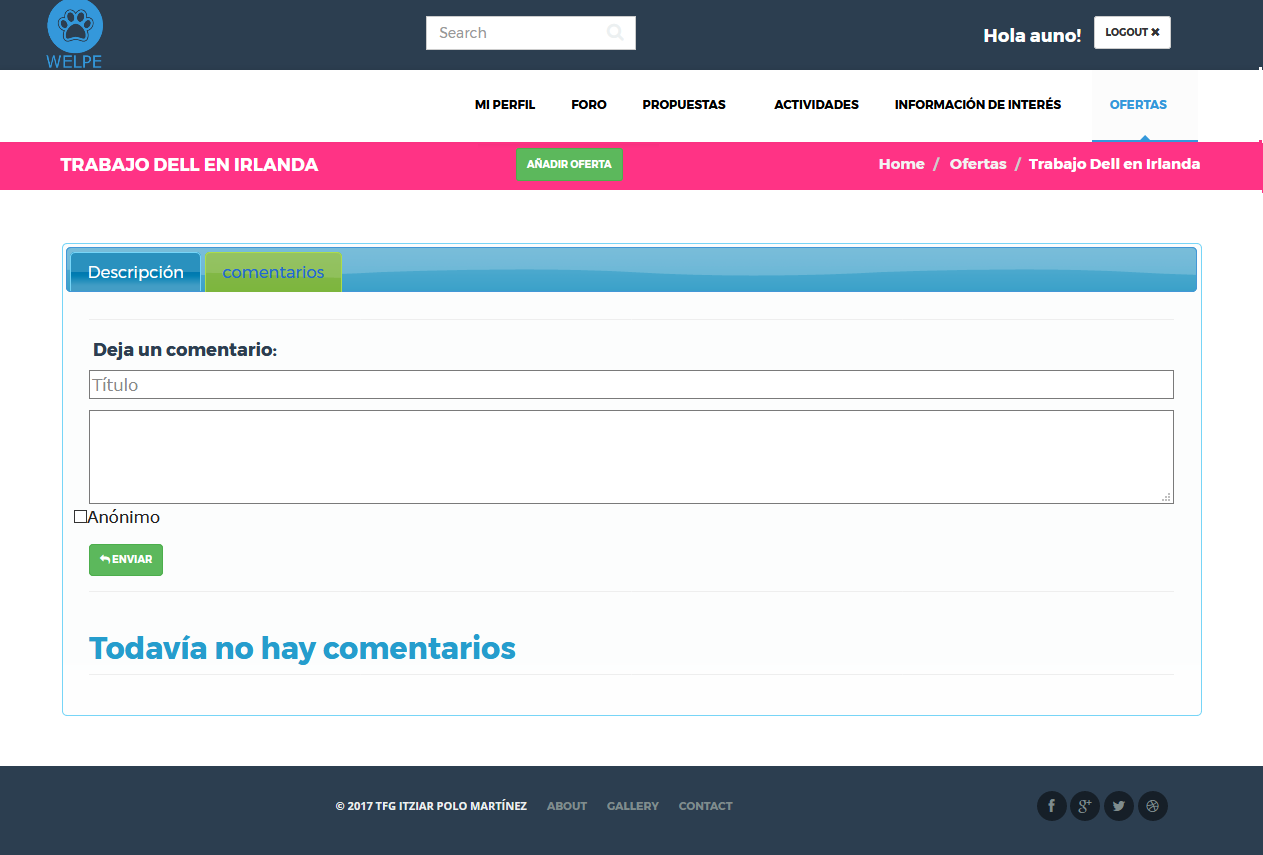
\includegraphics[width=12cm]{img/oferta_comment}
\caption{Vista de los comentarios a una oferta}
\label{figura:oferta_comment}
\end{figure}
La página de una oferta es enviada al cliente cuando se recibe una petición GET sobre el recurso /ofertas/{título\_oferta}\\
En esta vista se muestra toda la información relativa a la oferta previamente introducida a través del formulario comentado anteriormente. \\
Relativo a esta vista se encuentra el nombre, el tipo de contrato ofertado, número de comentarios, los comentarios, las veces que la oferta se ha guardado en la lista de favoritos, la descripción de la oferta, como aplicar a la oferta, etc.\\
En esta vista se puede interactuar de las siguientes formas sólo si el usuario registrado:
\begin{itemize}
\item Se puede crear una nueva oferta mediante el botón nueva oferta donde se abrirá un modal en el que se pedirán ciertos datos; este formulario ya cumplimentado se enviará al servidor donde se procesará y almacenara, devolviendo como resultado una nueva vista donde se muestra la oferta que el usuario previamente ha creado.
\item Si el usuario es el propietario de la oferta podrá modificarla mediante el botón edit y también podrá eliminarla mediante el botón eliminar.
\item •	Junto con todo ello, está también el botón de favoritos donde el usuario puede agregar o eliminar la oferta de su lista de favoritos.  
\item Se ha proporcionado un apartado de comentarios a la oferta para que los usuarios puedan comentar cada oferta.
\end{itemize}

\subsubsection{Página de Información de Interés}
\label{subsubsec:informaciones}
\begin{figure}[H]
\centering
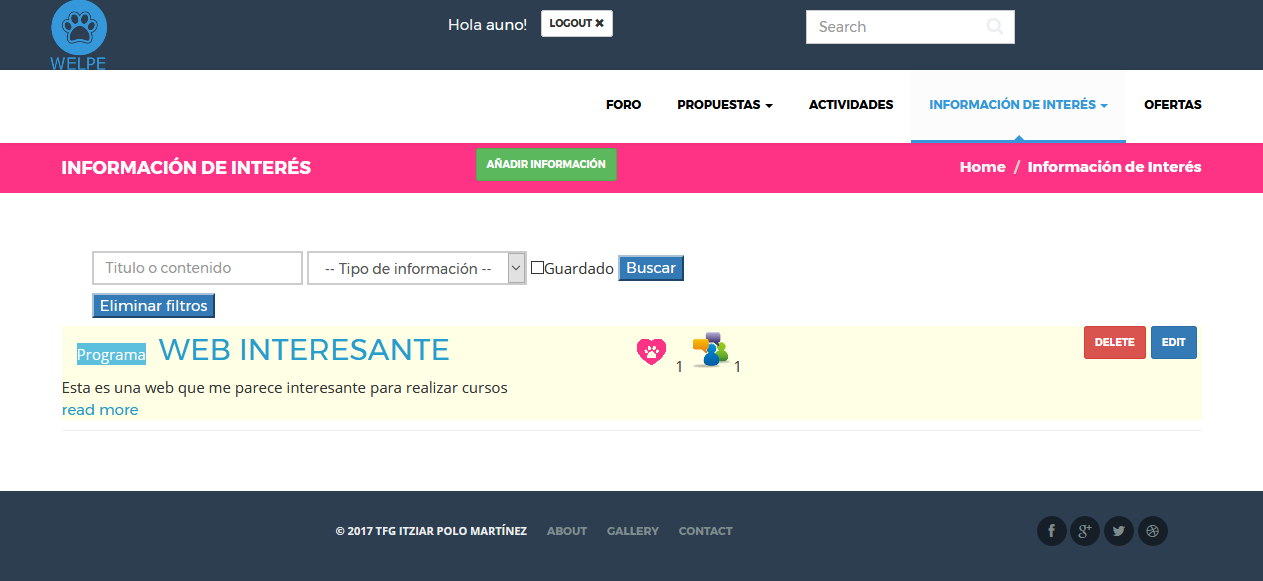
\includegraphics[width=12cm]{img/infos_interes}
\caption{Vista de la lista de informaciones de interés}
\label{figura:infos_interes}
\end{figure}
La página del listado de informaciones es enviada al cliente cuando se recibe una petición GET sobre el recurso /informacion.\\
En esta vista se muestra un listado con toda la información de las distintas informaciones de interés que se han ido recopilando junto con una pequeña parte de la descripción. Además a la izquierda del título se muestra la clase de información que ofrece y a la derecha se puede observar varios elementos. En primer lugar un corazón que viene a significar si la información de interés se ha guardado en la lista de favoritos o no, además de un número que irá creciendo o decreciendo dependiendo del número de usuarios que las guarden en sus listas de favoritos. A continuación se observa el número de comentarios que contiene cada información.\\
También cualquier usuario (registrado o no) puede filtrar este listado por la/s palabra/s que contenga el título o contenido de la información deseada, además también podemos filtrar por el tipo de información que se ofrece a elegir entre beca de estudios, programa, curso, concurso u otro tipo de información y además si el usuario está registrado podrá filtrar si la información está o no en su lista de favoritos.\\
Para introducir una nueva información cualquier usuario registrado puede hacerlo. Para ello se hace click en el botón “Añadir información” se rellena el formulario con los datos correspondientes y se envía. Esta petición llega al servidor mediante una petición POST donde se encargará de sacar los datos y guardarlos correctamente en la base de datos devolviendo como resultado una nueva vista donde se muestra la información de interés que el usuario previamente había enviado.\\
Por último, sólo si el usuario ha creado una determinada información de interés o es un profesor o es el administrador: podrá modificar y/o eliminar dicha información mediante los botones edit y delete.

\subsubsection{Página de una Información de interés }
\label{subsubsec:informacion}
\begin{figure}[H]
\centering
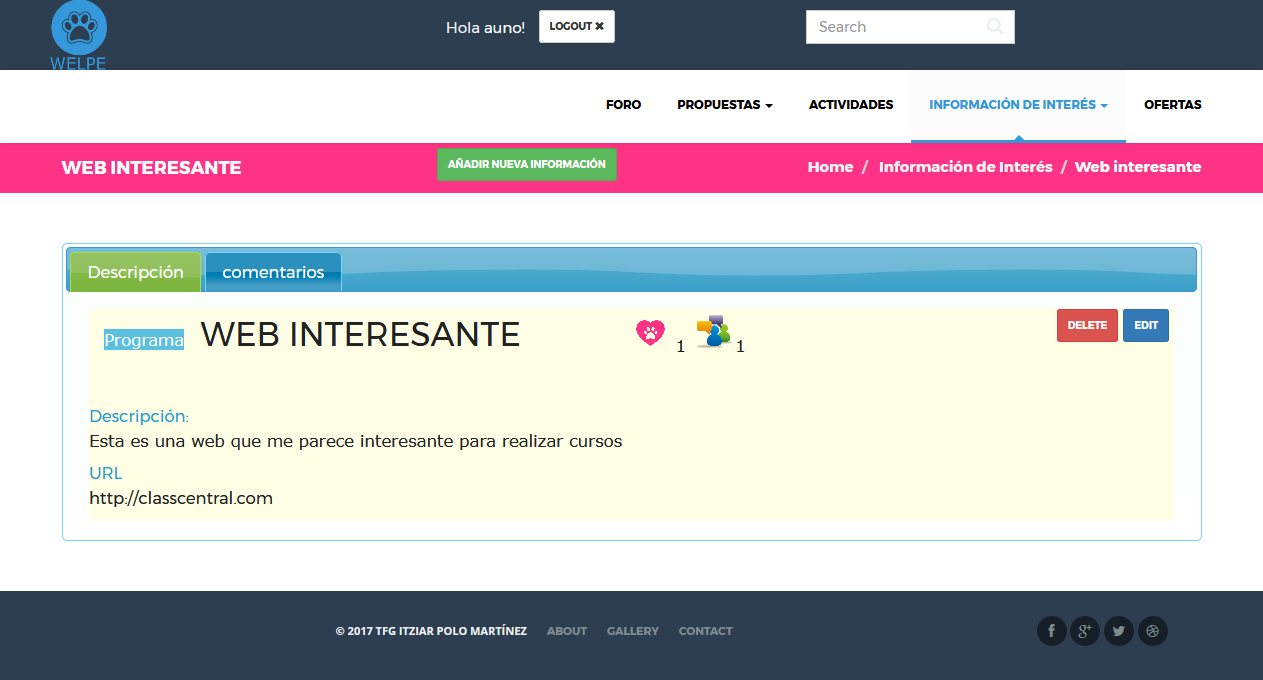
\includegraphics[width=12cm]{img/info_interes}
\caption{Vista de una información de interés}
\label{figura:info_interes}
\end{figure}
\begin{figure}[H]
\centering
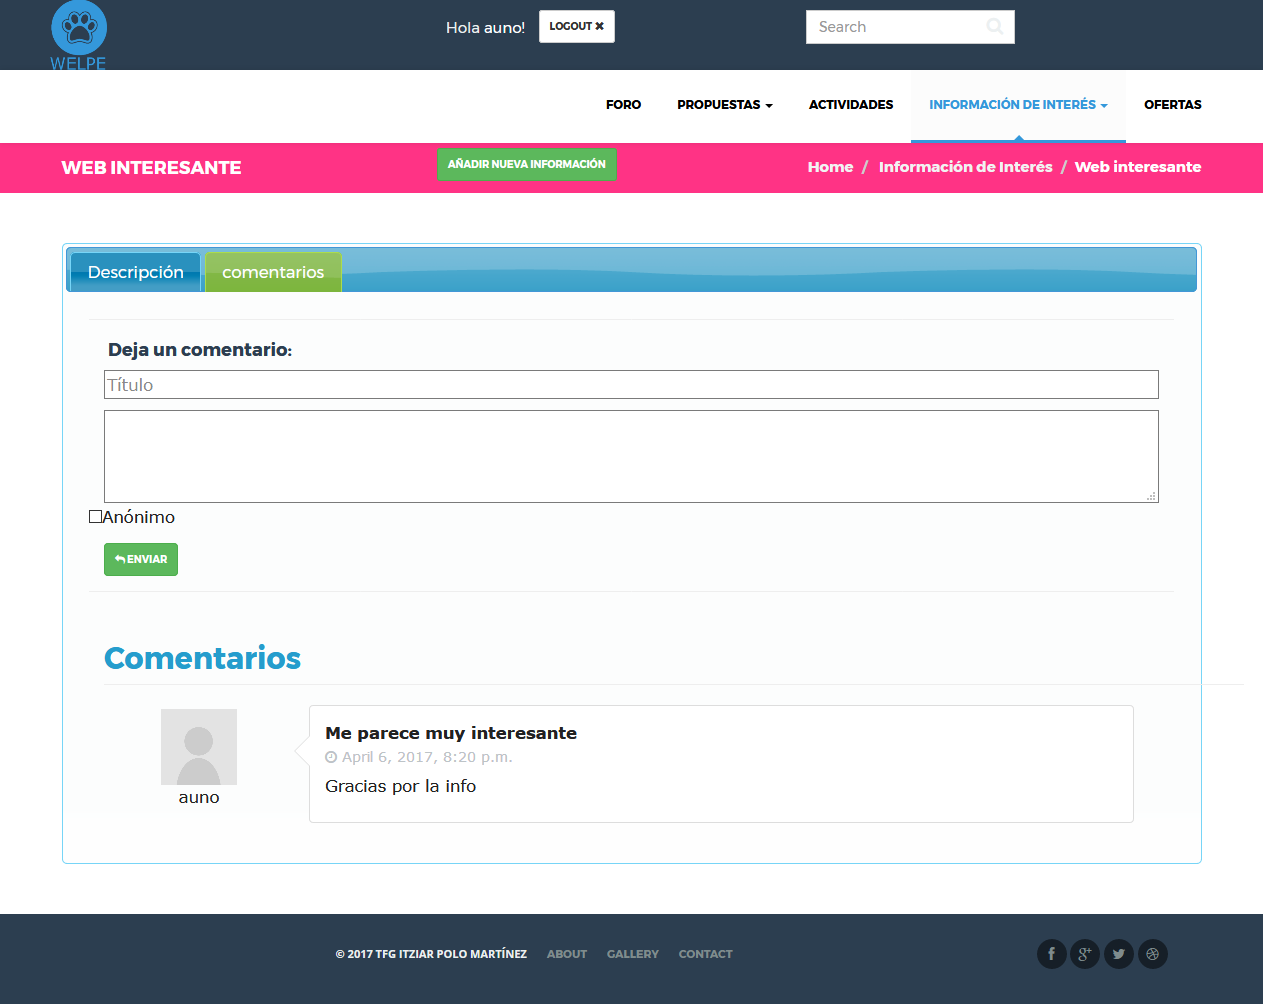
\includegraphics[width=12cm]{img/info_interes_comment}
\caption{Vista de los comentarios a una información de interés}
\label{figura:info_interes_comment}
\end{figure}
La página de una información es enviada al cliente cuando se recibe una petición GET sobre el recurso /informacion/{título\_información\_de\_interés}\\
En esta vista se muestra toda la información relativa a una única información de interés que previamente ha sido incluida a través del formulario comentado anteriormente. \\
Relativo a esta vista se encuentra el título, el tipo de información ofrecida, número de comentarios, los comentarios, las veces que dicha información de interés se ha guardado en la lista de favoritos, la descripción de la información, url donde encontrar más información, etc.\\
En esta vista se puede interactuar de las siguientes formas sólo si es un usuario registrado:
\begin{itemize}
\item Se puede crear una nueva información  mediante el botón añadir información donde se abrirá un modal en el que se pedirán ciertos datos, este formulario ya cumplimentado se enviará al servidor donde se procesará y almacenará devolviendo como resultado una nueva vista donde se muestra la nueva información de interés.
\item Si el usuario es el propietario de la información de interés podrá modificar mediante el botón edit, y eliminarla mediante el botón delete.
\item Junto con todo ello, está también el botón de favoritos donde el usuario puede agregar o eliminar dicha información de interés de su lista de favoritos.  
\item Se ha proporcionado un apartado de comentarios donde los usuarios pueden compartir sus opiniones y/o aclarar sus dudas acerca de la información de interés.
\end{itemize}

\subsubsection{Página de Política de Cookies}
\label{subsubsec:cookies}
Esta vista tiene que ver más con la legislación que con la propia aplicación.\\
El Real Decreto-ley 13/2012, de 30 de marzo, publicado en el «Boletín Oficial del Estado» el pasado sábado 31 de marzo de 2012, transpone la Directiva 2009/136/CE, del Parlamento Europeo y del Consejo, de 25 de noviembre de 2009, que se integra en la LSSI (Ley 34/2002, de 11 de julio, de servicios de la sociedad de la información y de comercio electrónico) modificando el punto segundo de su artículo 22, que queda redactado de la forma siguiente:\\
``Artículo 22.2 de la Ley 34/2002. Los prestadores de servicios podrán utilizar dispositivos de almacenamiento y recuperación de datos en equipos terminales de los destinatarios, a condición de que los mismos hayan dado su consentimiento después de que se les haya facilitado información clara y completa sobre su utilización, en particular, sobre los fines del tratamiento de los datos, con arreglo a lo dispuesto en la Ley Orgánica 15/1999, de 13 de diciembre, de Protección de Datos de Carácter Personal. Cuando sea técnicamente posible y eficaz, el consentimiento del destinatario para aceptar el tratamiento de los datos podrá facilitarse mediante el uso de los parámetros adecuados del navegador o de otras aplicaciones, siempre que aquél deba proceder a su configuración durante su instalación o actualización mediante una acción expresa a tal efecto. Lo anterior no impedirá el posible almacenamiento o acceso de índole técnica al solo fin de efectuar la transmisión de una comunicación por una red de comunicaciones electrónicas o, en la medida que resulte estrictamente necesario, para la prestación de un servicio de la sociedad de la información expresamente solicitado por el destinatario.''\\
Por si no hubiera quedado claro del todo nos podríamos enfrentar a distintas sanciones dependiendo de la gravedad que consideren:\\
- Sanción Leve hasta 30.000 Euros.  Art. 38.4 LSSI. Son infracciones leves:
g) ``El incumplimiento de las obligaciones de información o de establecimiento de un procedimiento de rechazo del tratamiento de datos, establecidas en el apartado 2 del artículo 22, cuando no constituya una infracción grave.''
- Sanción Grave de 30.000 hasta 150.000 Euros. Art. 38.3 LSSI. Son infracciones graves:
i) ``El incumplimiento significativo de las obligaciones de información o de establecimiento de un procedimiento de rechazo del tratamiento de datos, establecidas en el apartado 2 del artículo 22.''\\
Con lo cual lo más conveniente es informar al usuario para evitar posibles sanciones.
 \begin{figure}[H]
    \centering
    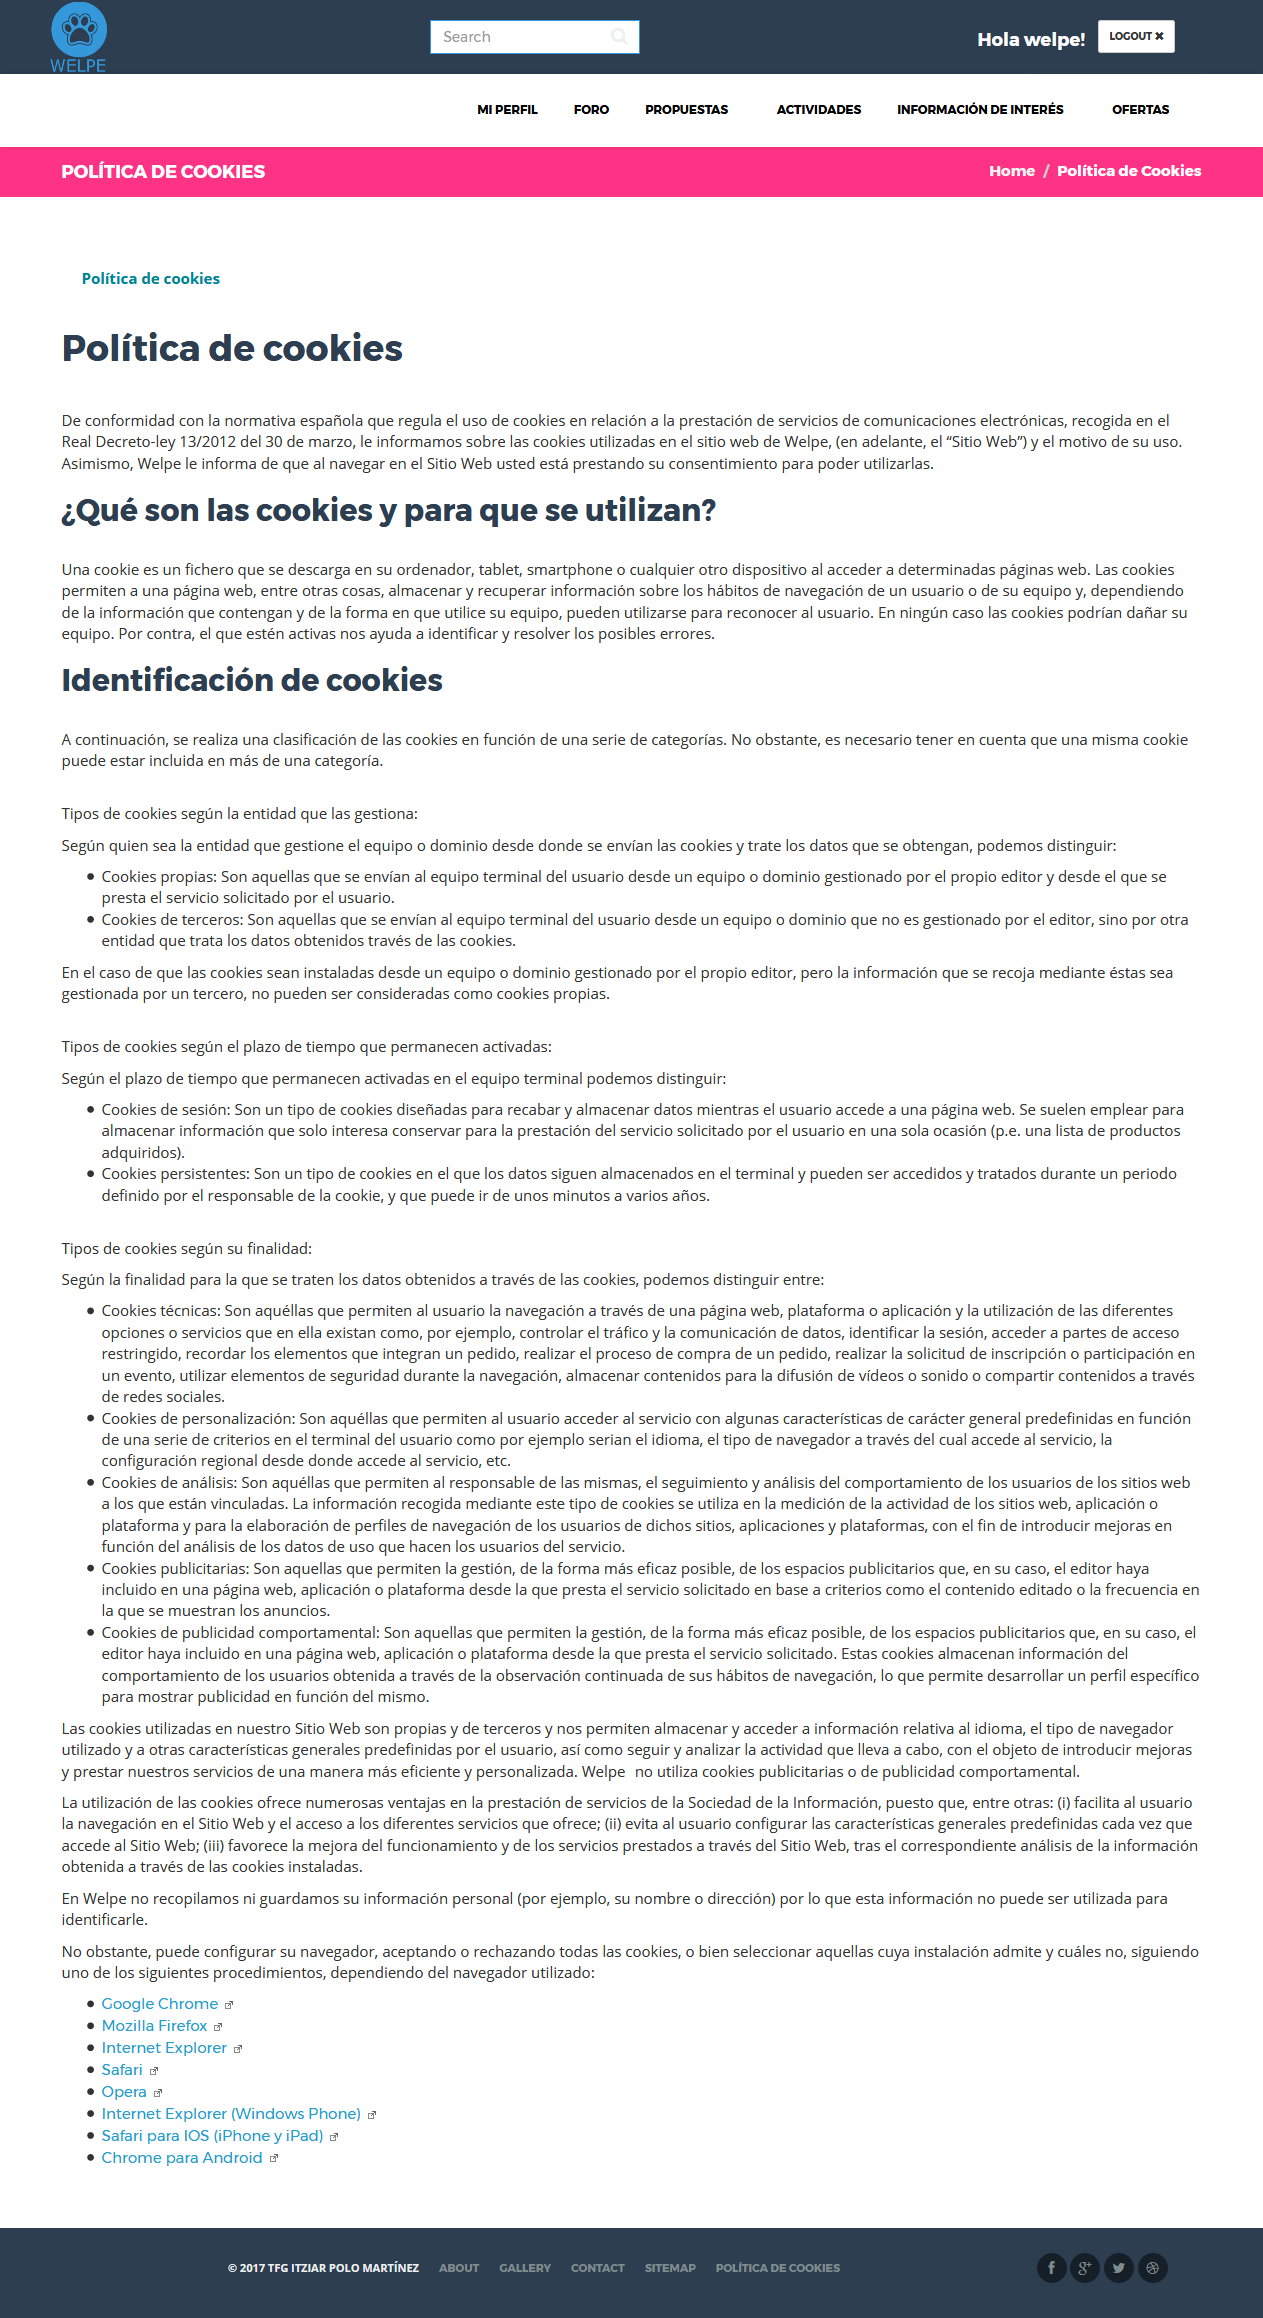
\includegraphics[width=12cm]{img/politica_cookies}
    \caption{Vista de la página política de cookies}
    \label{figura:politica_cookies}
 \end{figure}

\subsubsection{Páginas de Sitemaps}
\label{subsubsec:sitemap}
Para mejorar el posicionamiento SEO, una recomendación es  tener dos sitemaps, uno para los buscadores (se puede acceder a través de /sitemap.xml) y otro creado especialmente para la compresión humana (se puede acceder a través de /sitemap).\\
El primero de los sitemap (sitemap.xml) el cms que se utiliza (Mezzanine) lo crea por defecto.\\
El segundo (/sitemap), se ha creado especialmente una aplicación mostrar el recorrido del árbol.

\subsubsection{Vista del panel de administración}
\label{subsubsec:admin}
Mezzanine al igual que Django, ofrece unas vistas para administrar la base de datos que es muy útil y fácil de usar. Desde ahí se puede crear, modificar o eliminar cualquier elemento que se desee y hacer un seguimiento de la base de datos. \\
Cada aplicación creada en este proyecto junto con otras, que el propio CMS posee, se encuentran disponibles en la parte de administración.  \\
Podemos observar que además de las vistas explicadas anteriormente también podemos podemos crear otras que ya vienen predefinadas con Mezzanine como entradas para un Blog, un Page (que sería como una página simple).\\
Además tenemos otras configuraciones sobre la plataforma en sí, como las proporcionadas por los menus Site y Theme.\\
Esta vista sólo es accesible para los administradores de la plataforma. Se puede acceder a ella a través de /admin.
\begin{figure}[H]
   \centering
   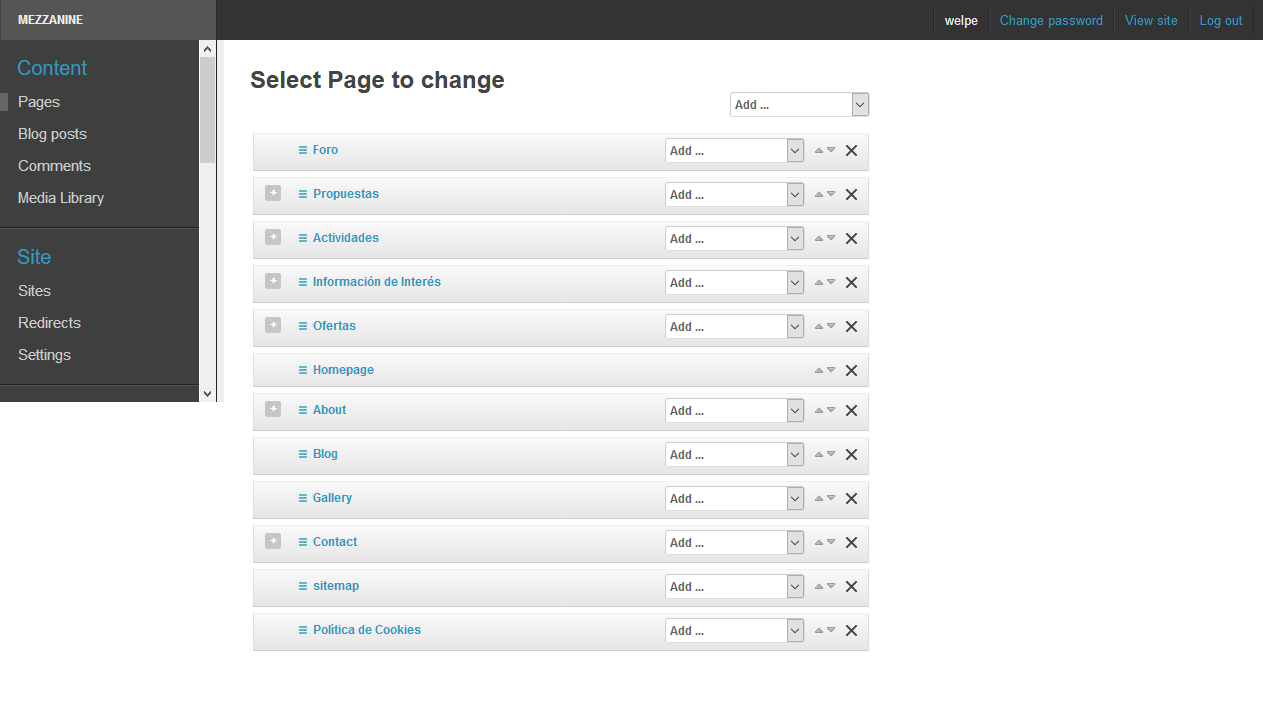
\includegraphics[width=12cm]{img/admin}
   \caption{Vista de la parte de administración}
   \label{figura:admin}
\end{figure}
\cleardoublepage
\chapter{Evaluación del resultado}
\label{chap:evaluation}


El presente proyecto pretendía ofrecer una nueva herramienta para la gestión y promoción de los distintos eventos fuera y dentro de la Universidad objetivo que se ha conseguido.


Analizando cada uno de los objetivos descritos en el capítulo 2 también obtenemos un resultado satisfactorio:


\begin{itemize}
\item Aplicación universal: se ha conseguido crear una aplicación compatible con los distintos dispositivos, sistemas operativos y navegadores web existentes. Además, también se adapta para ofrecer un control y apariencia adecuados independientemente del tipo de dispositivo utilizado.
\item Sencillez en su uso: se ha creado un interfaz sencilla e intuitiva para todos los usuarios. Además presenta una página de contacto para poder comunicarse con el/los administrador/es.
\item Gestionar y promocionar mejor las actividades para que los alumnos crezcan tanto a nivel personal como profesional.  Además de las distintas actividades en cada una de las secciones, se ha proporcionado una herramienta para que los alumnos puedan proponer sus propias actividades (dentro de la sección propuesta) y los profesores si lo ven viable, esas propuestas se conviertan en futuras actividades. Con esta herramienta conseguimos que los profesores puedan escuchar lo que los alumnos más demandan.
\item Web colaborativa: aunque de momento no hay muchos usuarios (los creados por mí), esta herramienta puede ser un complemento al actual Moodle o incluso en un futuro llegar a sustituirlo añadiendo más módulos. Actualmente esta aplicación cuenta con la gestión de todos los eventos que se quieren hacer llegar a los alumnos y además consiguiendo algo que muy pocas veces ocurre y es que los alumnos puedan proponer sus ideas y salgan adelante en forma de seminarios, cursos, etc.
\item Aportar un elemento social: se ha creado un foro para que todos los miembros de la universidad puedan comunicarse y colaborar para lograr un mejor entorno universitario. 
\item Uso de tecnologías web avanzadas: se han utilizado varias herramientas web como HTML5, CSS3, Python, Django, JS, etc. que juntándolas han propiciado un buen resultado final.
\end{itemize}


\cleardoublepage
\chapter{Conclusiones}
\label{chap:conclusiones}


\section{Conocimientos aplicados} 
\label{sec:aplicados}


Para el desarrollo del presente proyecto he utilizado los conocimientos adquiridos durante mi etapa en la Universidad cursando el Grado en Ingeniería en Tecnologías de la Telecomunicación.


Durante mi etapa en la universidad he crecido como profesional pero también como persona. Puedo decir que he adquirido gran cantidad de conocimiento, con lo cual quedarme con una sola asignatura para reflejar este proyecto sería un poco injusto; ya que de cada asignatura me llevo aunque sólo sea una pequeña parte y esa parte al final queda reflejada en lo que se hace día a día.


Si tuviera que destacar alguna o algunas asignaturas serían las orientadas en el área de programación puesto que su contenido y conocimiento se ajustan más al contexto del presente trabajo:



\begin{itemize}
\item Fundamentos de la Programación (FDP): es la asignatura que proporciona la base de la programación. Es donde ves por primera vez cómo se usa “eso de los ordenadores” y donde te dan ganas de salir corriendo (pero no lo haces).
\item Servicios y Aplicaciones Telemáticas (SAT): es la asignatura en que por primera vez ves que es útil eso de la programación y se pueden hacer cosas “chulas” e interesantes ya que en las anteriores asignaturas del área de programación eran mediante una terminal. En esta asignaturas aprendí Python, Django y también a crear webs. Con esta asignatura también descubrí que realmente sí que me gustaba programar (antes de esta asignatura, para mí, las asignaturas de esta área eran una continua tortura)
\item Ingeniería de Sistemas de Información (ISI): es la asignatura donde aprendes a desarrollar junto a tu equipo con herramientas que en el mundo profesional real se usan. A ver que hay vida más allá de las BBDD relacionales, etc. Aunque estas herramientas no las he usado en mi proyecto, las tengo muy presente en mi carrera profesional.
\item Desarrollo de Aplicaciones Telemáticas (DAT): es una asignatura donde aprendes a comunicarte (y sobre todo pegarte) con distintas APIS. 
\item Del resto de asignaturas me quedo con la capacidad de esfuerzo y entrega que he tenido, intentando dar al máximo en cada una de ellas, algunas veces viendo recompensa otras veces había que seguir intentándolo con mucho más empeño y esfuerzo.
\end{itemize}


También he aprendido bastante de los seminarios impartidos por profesores e incluso me ha tocado a mí dar alguno. En el que impartí sobre LaTeX, aprendí un poco más sobre esa herramienta que para muchos es desconocida además aprendí el trabajo y esfuerzo que hay al organizar un seminario que van más allá de una simple presentación.


Aunque no se promocione mucho, también he aprendido bastante en los diferentes cursos llamados MOOC (Massive Online Open Courses) que ofrecen las diferentes universidades del mundo y plataformas. Empezó siendo un entretenimiento y al final se convirtió en un apoyo para mis estudios (aunque hubiera cursado alguno que no fuera directamente de la rama ‘Computer Science’). Con estos cursos además del propio contenido y de inglés, he aprendido a abrir mi mente y no estar encerrada en mi burbuja.


Quiero terminar este apartado con una GRACIAS a todos y cada uno de los profesores. De cada uno de vosotros me llevo una parte, tanto personal como profesionalmente. Seguro que aplicaré todos estos conocimientos proporcionados a lo largo de mi carrera profesional.



\section{Conocimientos adquiridos} 
\label{sec:adquiridos}

Durante la realización de este proyecto, no sólo he aprendido a poner en práctica mis conocimientos adquiridos durante la carrera, sino que este trabajo me ha permitido adquirir nuevos conocimientos y experiencias.


Al iniciar este trabajo, no me había enfrentado anteriormente a la creación de una aplicación de tal envergadura. Sin embargo, me he demostrado que mis conocimientos adquiridos durante la carrera (esfuerzo y constancia) estaban ahí que por mucho que diga “no puedo más” o “no lo voy a conseguir” siempre voy un poco más allá y siempre doy ese último pequeño esfuerzo.


En cuanto a mis conocimientos, he solidificado y madurado mis conocimientos en todas las tecnologías utilizadas y descritas en el capítulo 3.


También he aprendido sobre el mundo de los gestores de contenido. Lo útiles que pueden llegar a ser y lo rápido que crecen hoy en día.


Para el desarrollo he utilizado el idle PyCharm y he decir que es una gran ayuda a la hora de depurar código y sobre todo a la hora de formatearlo (seguro que he infrautilizado este idle pero en un futuro pienso utilizarlo mucho más).


Al decidirse desplegarlo en la nube, he adquirido conocimientos en cloud que seguro serán muy útiles en mi carrera profesional, además también me incita a aprender un más sobre este tema tan de moda y tan olvidado en la universidad. 



\section{Trabajos futuros} 
\label{sec:futuro}


\begin{itemize}
\item Autenticación mediante LDAP de la Universidad
\item Ampliación de esta aplicación con nuevas sub-aplicaciones para poder ser más completo y que en un futuro pueda sustituir a Moodle o al menos que puede equipararse al nivel de Moodle.
\item Mejor eficiencia: siempre puede mejorarse la eficiencia de la aplicación, y debería mejorarse sobre todo las peticiones a la base de datos para así tener una mayor velocidad de navegación. 
\item Aplicación móvil: una aplicación móvil que ofrezca todas las funcionalidades que ofrece la aplicación web. Los dispositivos móviles son muy usados por cualquier persona joven y podría llegar a más alumnos. Para los más tradicionales, en cuanto a tecnologías se refiere, seguiría teniendo la aplicación web.
\end{itemize}



%%%%%%%%%%%%%%%%
% BIBLIOGRAFIA %
%%%%%%%%%%%%%%%%
\cleardoublepage

\begin{thebibliography}{25}
\bibliographystyle{alpha}

\bibitem{jQuery} Página oficial de jQuery.    \\
{\footnotesize \url{http://jquery.com/}}

\bibitem{JSON} Página sobre JSON.    \\
{\footnotesize
\url{http://www.json.org/}}


\bibitem{Bootstrap} Página oficial de Bootstrap.    \\
{\footnotesize
\url{http://getbootstrap.com/}}

\bibitem{Python} Página oficial de Python.     \\
{\footnotesize
\url{https://www.python.org/}}

\bibitem{Django} Página oficial de Django.      \\
{\footnotesize
\url{https://docs.djangoproject.com/}}

\bibitem{normas_estilo} Página con las normas de estilo de Python     \\
{\footnotesize
\url{http://legacy.python.org/dev/peps/pep-0008/}}

\bibitem{Mezzanine} Página oficial de Mezzanine.   \\
{\footnotesize
\url{http://mezzanine.jupo.org/}}

\bibitem{PyCharm} Página oficial de PyCharm    \\
{\footnotesize
\url{https://www.jetbrains.com/pycharm/}}

\bibitem{HTML5} Página sobre HTML5.    \\
{\footnotesize
\url{http://www.w3schools.com/html/html5_intro.asp}}

\bibitem{CSS3} Página sobre CSS3.    \\
{\footnotesize
\url{http://www.w3schools.com/css/css3_intro.asp/ }}

\bibitem{cookies} Información sobre la legislación española respecto a la política de cookies      \\
{\footnotesize
\url{http://politicadecookies.com/sanciones.php}}

\bibitem{AWS}[Amazon Web Service versión estudiantes
{\footnotesize
\url{https://aws.amazon.com/es/education/awseducate/ }}

\end{thebibliography}

\cleardoublepage
\appendix
\chapter{Instalación y Uso}
\label{app:instalacion}


Para el funcionamiento de la aplicación lo primero que hay que hacer es instalar todos los paquetes necesarios. Estos paquetes se encuentran en el archivo ``requirements.txt''. Por lo tanto con ejecutar en una \textit{shell} ``pip install –r requirements.txt'' se instalaran los paquetes necesarios, sino es que ya están instalados en la máquina.


Una vez instalados, ejecutar en una \textit{shell} el comando ``python manage.py createdb'', que creará una base de datos, creando además un superusuario-administrador. A continuación hay que ejecutar el comando ``python manage.py runserver''. Cuando la aplicación esté en funcionamiento nos dirá tanto la IP como el PUERTO, por defecto localhost 8000. Se abrirá un navegador web donde habrá que introducir la URL ``htttp://localhost:8000''

\cleardoublepage
\chapter{Publicación}
\label{app:publicacion}

La aplicación se encuentra publicada en: 
\url{http://ec2-54-71-52-158.us-west-2.compute.amazonaws.com/}
La cual estará disponible durante el año 2017.


El código fuente se encuentra disponible en:
\url{https://github.com/itziar/Welpe/}


La presente memoria se encuentra disponible en:
\url{https://github.com/itziar/TFG-Memoria/}





\end{document}
